%%%%%%%%%%%%%%%%%%%%%%%%
%
% $Autor: Wings $
% $Datum: 2019-07-09 09:26:07Z $
% $Pfad: Vorlesungen/WS_19_20/Projekte/KandaNeuralnetwork/latex - Ausarbeitung/Kapitel/Hardware.tex $
% $Version: 4440 $
%
%%%%%%%%%%%%%%%%%%%%%%%%





\section{Portenta H7 - Hardware}

The Arduino portenta H7 can simultaneously execute high-level code together with real time task. For instance, one core reads data from sensors or other devices and the other core could be used for applying machine learning techniques from the acquired data. It has two 80-pin high density connectors which enables scalability for different applications by just attaching the board with other compatible boards like Vision shield.\cite{PortentaH7:2021}
\vspace*{-\baselineskip}

\begin{table}[h]
	\centering
	\caption{Specifications Table}
	\label{table1}
	\begin{tabular}{|p{5cm}| p{10cm} |} 
		\hline
		\textbf{Main Processor} & STM32H747XI dual Cortex\textregistered-M7+M4 32bit low power Arm\textregistered MCU \\ \hline 
		\textbf{SDRAM} & 8-64 MByte option \\ \hline
		\textbf{QSPI Flash}	& 2-128 MByte option \\ \hline
		\textbf{Ethernet}	& 10/100 Phy option\\ \hline
		\textbf{Wireless} & BT5.0 + WiFi 802.11 b/g/n 65Mbps option\\ \hline
		\textbf{Crypto chip}	& ECC608 or SE050C2 (Common Criteria EAL 6+) option\\ \hline
		\textbf{Display Connector}	& MIPI DSI host and  MIPI D-PHY to interface with low-pin count large displays \\
		\hline
		\textbf{GPU} & Chrom-ART graphical hardware Accelerator \\ \hline
		\textbf{Timers}	& 22x timers and watchdogs \\ \hline
		\textbf{UART}	& 4x ports (2 with flow control)\\ \hline
		\textbf{SD Card}	& 	Interface for SD Card connector (through expansion port only)\\ \hline
		\textbf{Operational Temperature}	& $-40^\circ$C to $+85^\circ$C \\ \hline
		\textbf{Power} & Through USB-C connector or LiPo battery (integrated charger) \\ \hline
		\textbf{Current Consumption} & 2.95 micro-Ampere in Standby mode (Backup SRAM OFF, RTC/LSE ON) \\ 
		\hline
		\textbf{USB-C} & Host / Device, DisplayPort out, High / Full Speed, Power delivery \\ \hline
		\textbf{MKR Headers} & Use any of the existing industrial MKR shields on it \\ \hline
		\textbf{High Density Connectors}	& Two 80 pin connectors will expose all of the board's peripherals to other devices \\ \hline
		\textbf{ESLOV Connector}	& Arduino's open connector standard for self-identifiable hardware \\ \hline
		\textbf{Camera Interface} &	8-bit, up to 80 MHz \\ \hline
		\textbf{ADC} & 3 $\times$ ADCs with 16-bit max. resolution (up to 36 channels, up to 3.6 MSPS) \\ \hline
		\textbf{DAC} & 2 $\times$ 12-bit DAC (1 MHz) \\ \hline
	\end{tabular}
\end{table} 
\vspace{-1.2cm}
\begin{figure}[H]
	\centering
	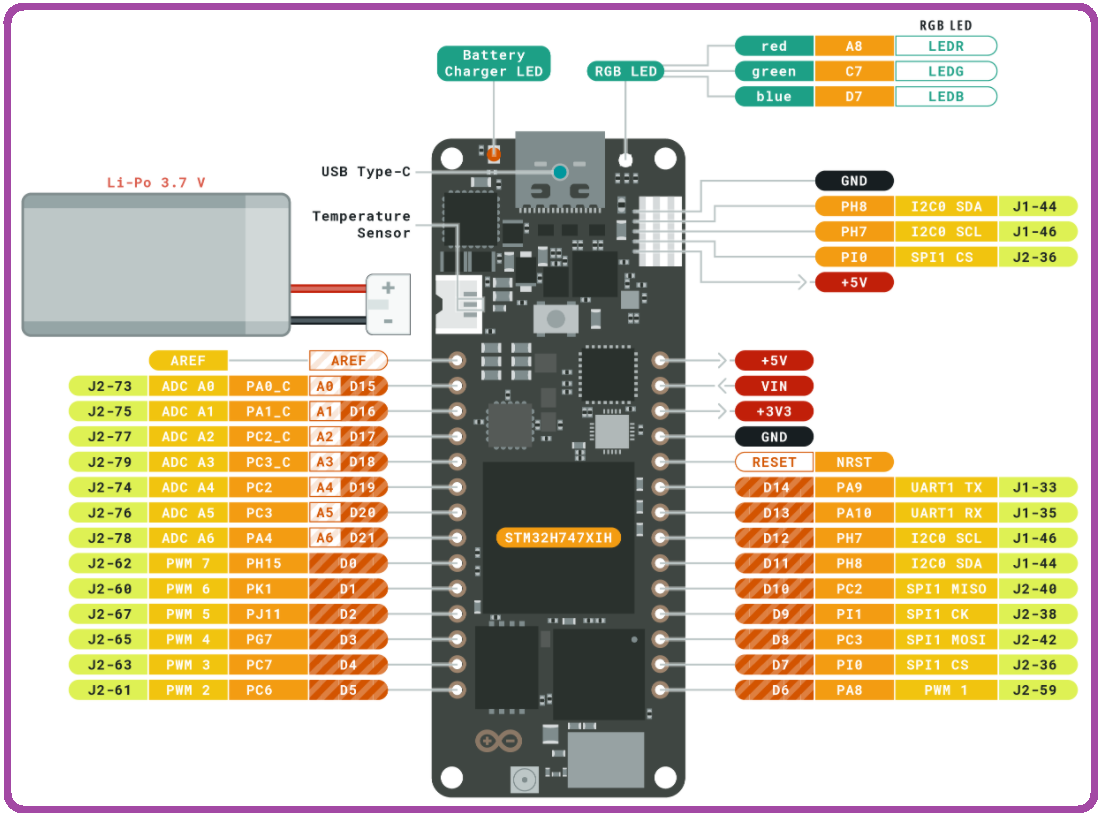
\includegraphics[width=150mm]{Arduino/basicportentapinout}
	\caption{Arduino Portenta  \href{https://store.arduino.cc/portenta-h7}{Arduino Store}}\label{figure 3.1}
\end{figure}

The above figure\ref{figure 3.1} represents the Arduino Portenta H7 board layout.  It has on the top a USB type-c connector along with two LEDs on its sides. One represents a battery charger LED which blinks while charging and the other LED glows when the Arduino Portenta is powered and ready to go. In addition to this, it has a temperature sensor and a blue reset button in the middle which resets the board. As can be seen from the figure, the pins A0 to A6 represents analog pins and D0 to D14 represents the digital pins.  The RGB LED present on top of the board is useful while programming by changing the colors to represent different outputs. The notations to use in the Arduino sketches for the LED colors are represented as LEDB for blue, LEDG for green and LEDR for red. The ground pins (GND) are denoted in black color and power pins in red color. VIN is the input voltage pin. This pin is used to power the board when the USB source is disconnected.  The 3v3 represents 3.3 volts output voltage pin and +5V pin is also a output voltage pin which outputs 5V from the board when powered using USB source or using the VIN pin. The SWD pin is a Serial Wire Debug pin which is used for debugging. On the back of the board, there are two 80-pin high density connectors to connect other boards.The pins for high density connectors are denoted as J1,J2 in the figure.\ref{figure 3.1}.There are PWM(Pulse Width Modulation) pins also present on the Arduino Portenta H7 board which are used in analog output demonstration like fading an LED.The ADC pins converts the analog input signal to digital output.It also has UART pins for communciation with other serial devices. Apart from this, it also has I2C(Inter Integrated Circuit) port at the top right  for communication between integrated circuits on the Arduino Portenta H7 board.


\section{Tutorial}


\begin{itemize}
  \item \url{https://store.arduino.cc/portenta-h7}
  \item \url{https://www.digikey.de/product-detail/de/arduino---bcmi-us-llc/ABX00042/1050-ABX00042-ND/11657626?utm_adgroup=Evaluation%20Boards%20-%20Embedded%20-%20MCU%2C%20DSP&utm_source=google&utm_medium=cpc&utm_campaign=Google%20Shopping_Development%20Boards%2C%20Kits%2C%20Programmers_New&utm_term=&productid=11657626&gclid=EAIaIQobChMIgprd57bO6gIVCJzVCh2plwHSEAkYAiABEgJ8xvD_BwE}
  \item \url{https://www.robotshop.com/de/de/arduino-portenta-h7-32-bit-arm-microcontroller.html?utm_source=google&utm_medium=surfaces&utm_campaign=surfaces_across_google_dede&gclid=EAIaIQobChMIgprd57bO6gIVCJzVCh2plwHSEAkYASABEgLvtfD_BwE}
  \item \href{https://www.arduino.cc/pro/tutorials/portenta-h7/por-ard-gs}{Tutorial}
\end{itemize}


\section{Hardware Installation}
To use the Arduino Portenta H7 we need to power it by connecting it to the PC by a USB type-C cable or by connecting a battery to the slot provided on the board. It supports single cell Li-po or Li-Ion battery(3.7V).  Here, we are going to connect the Arduino portenta H7 to a host laptop.
Hardware and software requirements :
\begin{itemize}
	\item	Arduino Portenta H7 board
	\item	USB type- C cable
	\item	Arduino IDE 1.8.10 or newer version
\end{itemize}
To start with, we connect the board to the laptop using a USB C cable. The LED on the board starts blinking green when its connected to the laptop. In case the board doesn?t respond via USB we can double press the reset button  and it enters into bootloader mode and the LED starts to blink again indicating it as ready. 
In order to use Arduino vision shield, we should connect it to the Arduino Portenta H7 using the high density connectors. The Arduino vision shield is designed to sit on top of the Arduino Portenta boards

\chapter{General Description of Softwares used in this project}
\section{Introduction}
In this chapter we will be going through the description of the Arduino IDE and describe  the features of it and what are all the options present in the IDE and how can we use it. Further we will be describing about the installation procedure of the Arduino IDE and how to get started with it.
\section{Arduino IDE Description}
It is an open source official Arduino software which used for editing, uploading and compiling codes in to the Arduino module. It is a cross-platform software which is available for Operating Systems like Windows, Linux, macOS. It runs on Java platform and supports a range of Arduino modules. It supports C and C++ languages. The microcontrollers present on the Arduino boards are programmed which accepts the information in the form of code. The program written in the IDE is called a sketch which will generate a Hex file which is then transferred and uploaded in the controller. The IDE environment is made up of two parts: an editor and a compiler. The editor is used to write the required code, while the compiler is used to compile and upload the code to the Arduino Module.\cite{Fezari:2018}

The Menu bar has options such as File in which there are many options including Opening a new file or existing,  Examples-in which we can find sketches for different applications like Blink, Fade etc.  There is an error console at the bottom  of the screen for displaying errors. 
\begin{figure}[H]
	\centering
	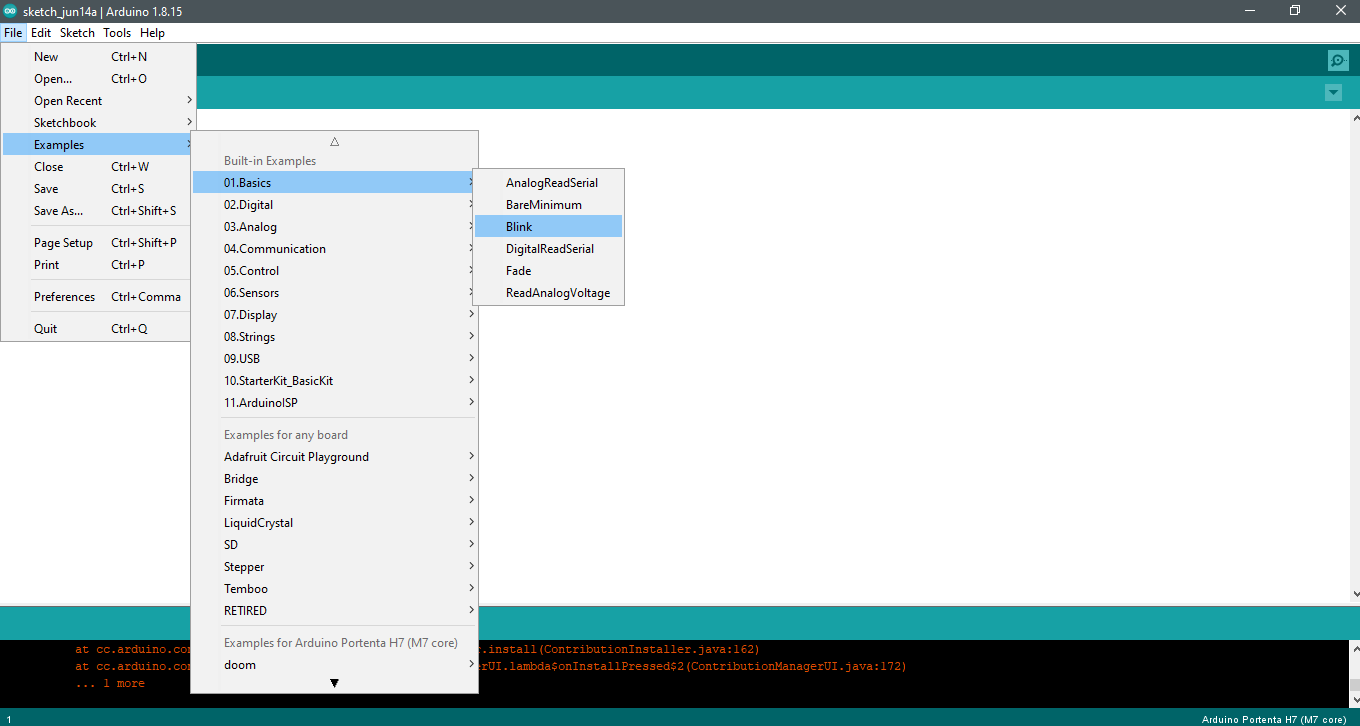
\includegraphics[width=0.9\textwidth]{Arduino/examplesketch}
	\caption{Menu bar options}\label{figure 4.1}
\end{figure}

The 6 buttons are present on top of the screen are as follows
\begin{figure}[H]
	\centering
	
\includegraphics[width=0.9\textwidth]{Arduino/menubar}
	\caption{Menu butons}\label{figure 4.2}
\end{figure}
\begin{itemize}
	\item	The check mark is used to verify your code. Click this once you have written your code.
	\item	The arrow uploads your code to the Arduino to run.
	\item	The dotted paper will create a new file.
	\item	The upward arrow is used to open an existing Arduino project.
	\item	The downward arrow is used to save the current file.
	\item	The far right button is a serial monitor, which is useful for sending data from the Arduino to the PC for debugging purposes.
\end{itemize}

\section{Installation}

To install the Arduino IDE, we need to download the latest version from the Arduino webpage \url{https://www.arduino.cc/en/software}. We can select the version based on the operating system we are using. Here we are installing Arduino 1.8..15 for a Windows 10 operating system. 
The set up file name is arduino-1.8.15-windows.exe and the size of it is 1,17,470 KB. we can specify the path according to our needs. Here i have set the path as \SHELL{C:/Program Files (x86)/Arduino}

After the download is done, open the setup file and proceed to install.
Select all the components in the dialog box and click Next.

\begin{figure}
	\centering
	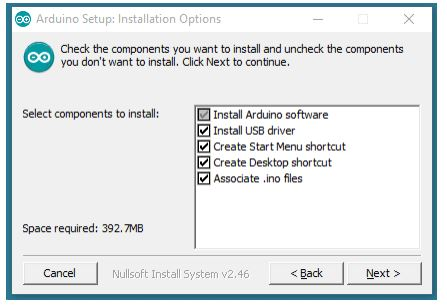
\includegraphics[width=0.7\textwidth]{Arduino/arduinoinst1}
	\caption{Arduino Setup Installation options}\label{figure 4.3}
\end{figure}

Select the destination folder and click Install

\begin{figure}
	\centering
	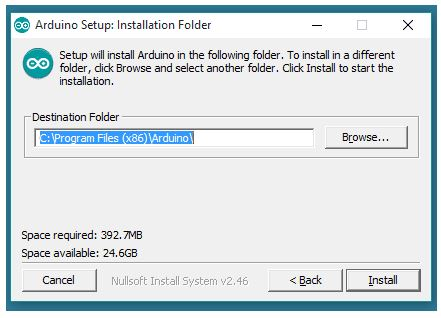
\includegraphics[width=0.7\textwidth]{Arduino/ardinst2}
	\caption{Arduino Setup: Installation Folder}\label{figure 4.4}
\end{figure}

Once the installation is done, open the Arduino IDE and a default sketch appears on the screen as shown.

\begin{figure}
	\centering
	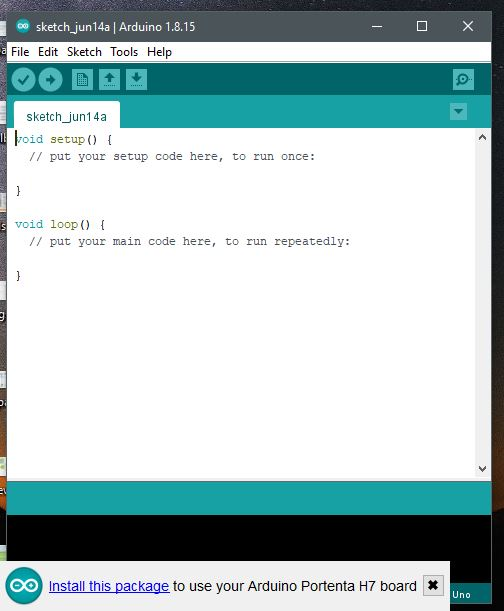
\includegraphics[width=0.7 \textwidth]{Arduino/arduinoidefrst}
	\caption{Arduino Sketch}\label{figure 4.5}
\end{figure}

It can be seen from the figure \ref{figure 4.5} that the basic arduino sketch has two parts. The first part is a void setup() function which returns void and we do the intiliaztion such as the output LED color, specifying the core etc. The second part is the void loop() function where we define functions which are to be performed through out the loop. These codes are placed between paranthesis{} and each function has a return type, here it has void return type.
\vspace{-0.6cm}



\chapter{First Steps with the Portenta H7}

\section{Introduction}

In this chapter we will be looking at how to connect the Arduino Portenta H7 with a PC/laptop  in order to use the board. Then, we will be going through the first steps of installing the relevant packages to use the Arduino Portenta H7 board and then we will be implementing a basic example sketch from the Arduino IDE.

\section{Configuration}
Connect the Arduino Portenta H7 board to the computer via USB Type-C cable. Press the reset button twice on the board and the LED on the board starts blinking green as shown in the figure \ref{figure 5.1} indicating that it is ready.

\begin{figure}
	\centering
	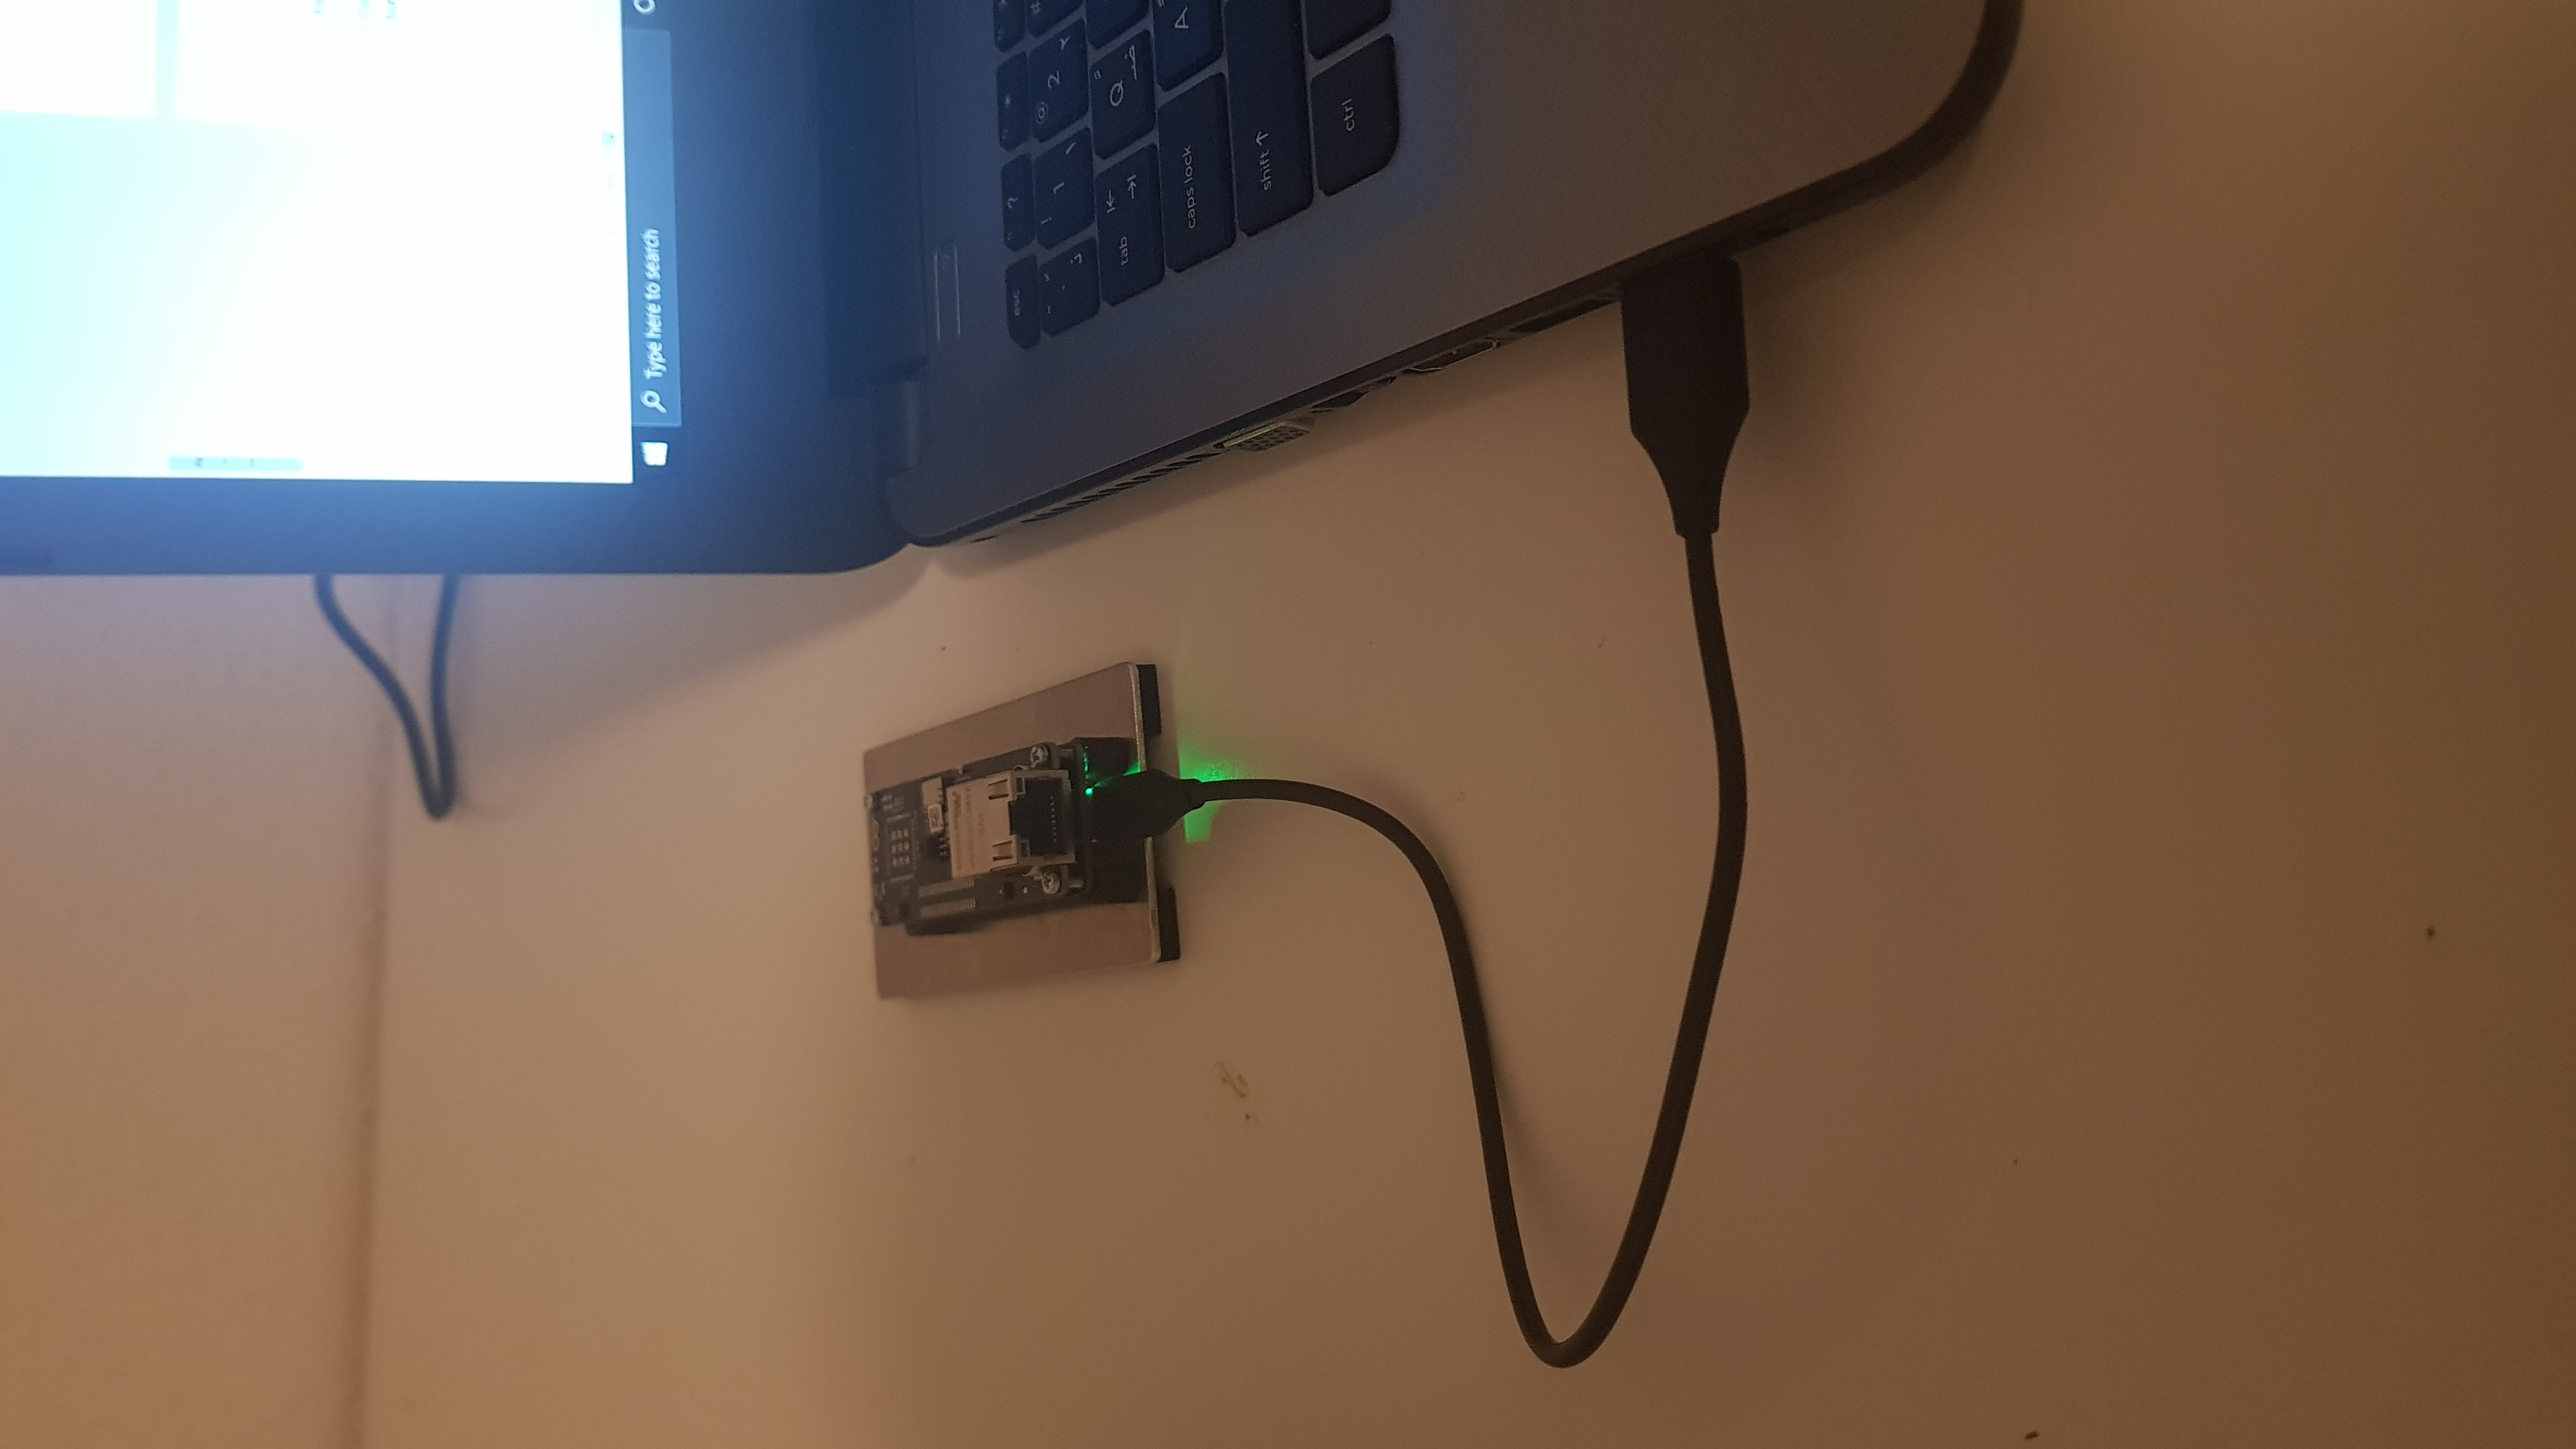
\includegraphics[width=0.9\textwidth,angle=-90]{Arduino/startinled}
	\caption{Arduino Portenta H7 Connected to a laptop  }
	\label{figure 5.1}
\end{figure}
First we need to install the packages in order to use the Arduino Portenta board. To do this search for Portenta in the boards and select Arduino Mbed OS Portenta Boards and click install as shown in figure \ref{figure 5.2}. After the installation is done, we can start writing sketches in the IDE.
\begin{figure}[H]
	\centering
	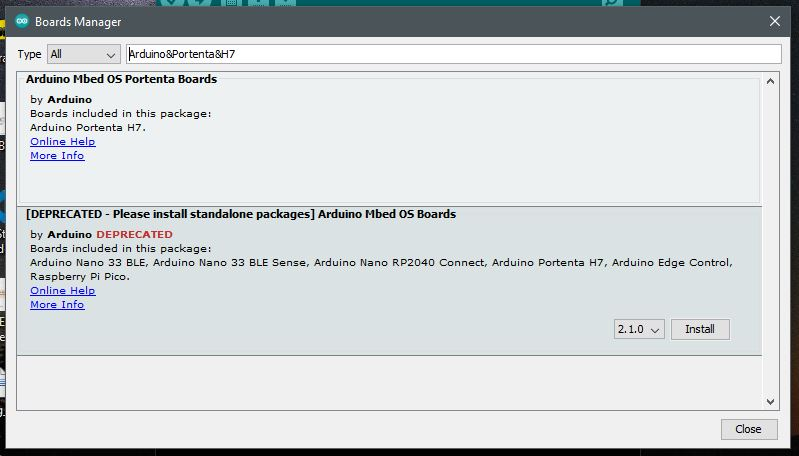
\includegraphics[width=0.8\textwidth]{Arduino/ardportinst}
	\caption{Install packages for Arduino Portenta H7}
	\label{figure 5.2}
\end{figure}
\subsection{Example Blink Sketch}
To upload the example sketch, go to File then click on examples and then click on 01.Basics and then select blink as shown in figure \ref{figure 5.3}.
\begin{figure}[H]
	\centering
	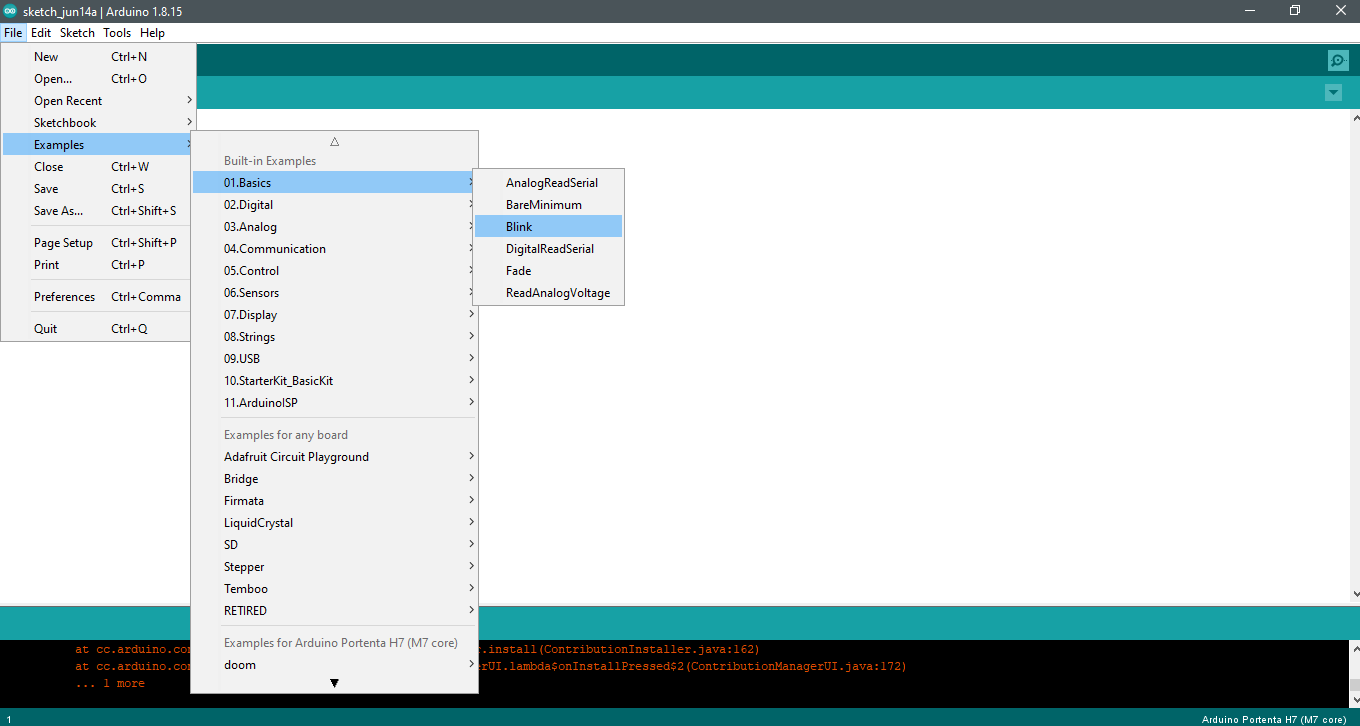
\includegraphics[width=0.8\textwidth]{Arduino/examplesketch}
	\caption{Upload Basic Sketch}
	\label{figure 5.3}
\end{figure}

In the program, we initialize LED\_BUILTIN as the output in the setup function. In the loop function   we turn on the LED by using digitalWrite() function. Click on upload and wait for it to complete. After the upload is done, the green LED on the board starts blinking with a delay of 1000ms.The blink sketch appears on the screen as shown in figure \ref{figure 5.4}.


\begin{figure}[H]
	\centering
	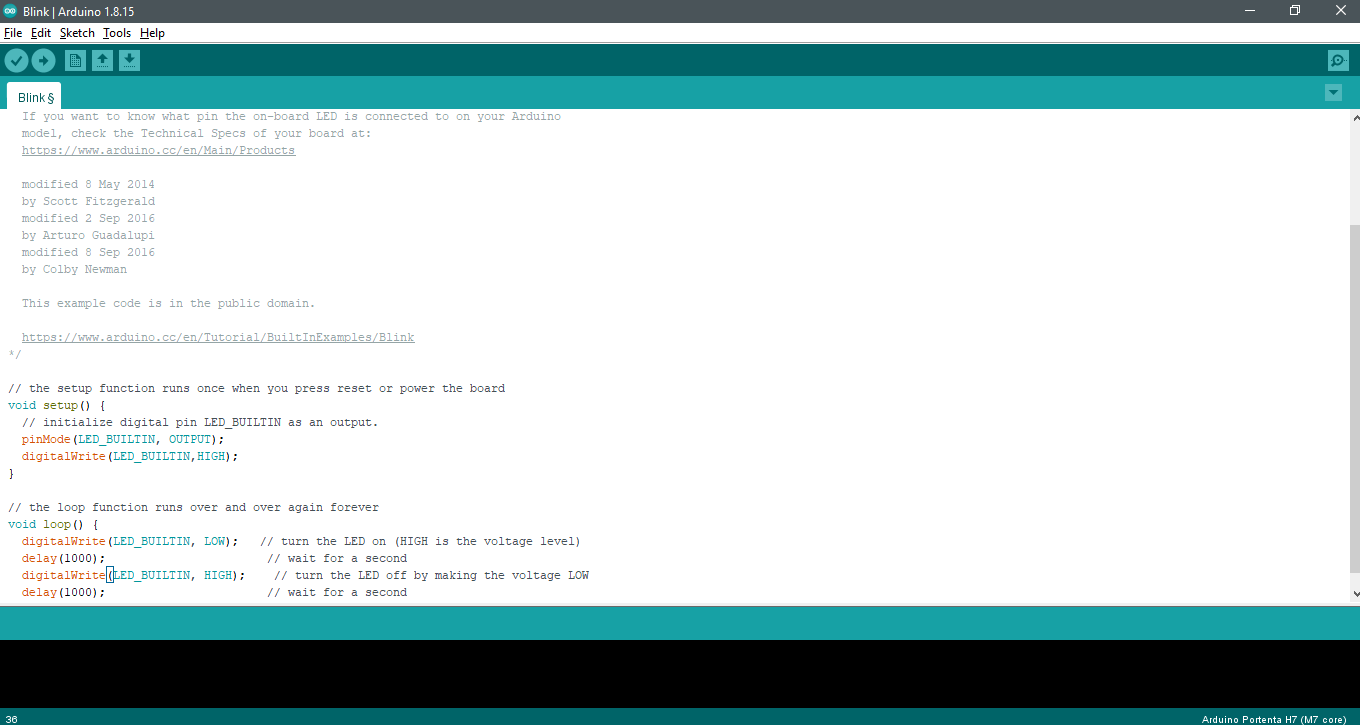
\includegraphics[width=0.8\textwidth]{Arduino/blinksketch}
	\caption{Compile Blink Sketch}
	\label{figure 5.4}
\end{figure}
.
\subsection{Serial Blink Example for Dual Core Processing}

The following figure~ \ref{figure 5.5} represents the serial blink sketch. This sketch helps in demonstrating the serial data transmission by showing the LED blinking after a certain time period. 

Here, Serial.begin(115200) command sets the data transmission rate to 115200 bits per second. The LEDB is the output which blinks in blue color and we have specified core M7. If we would like to use core M4 then we need to boot it first using bootM4() command. The ouput LED blinks blue in color after a delay of 3 seconds as defined in the sketch.
\begin{figure}[H]
	\centering
	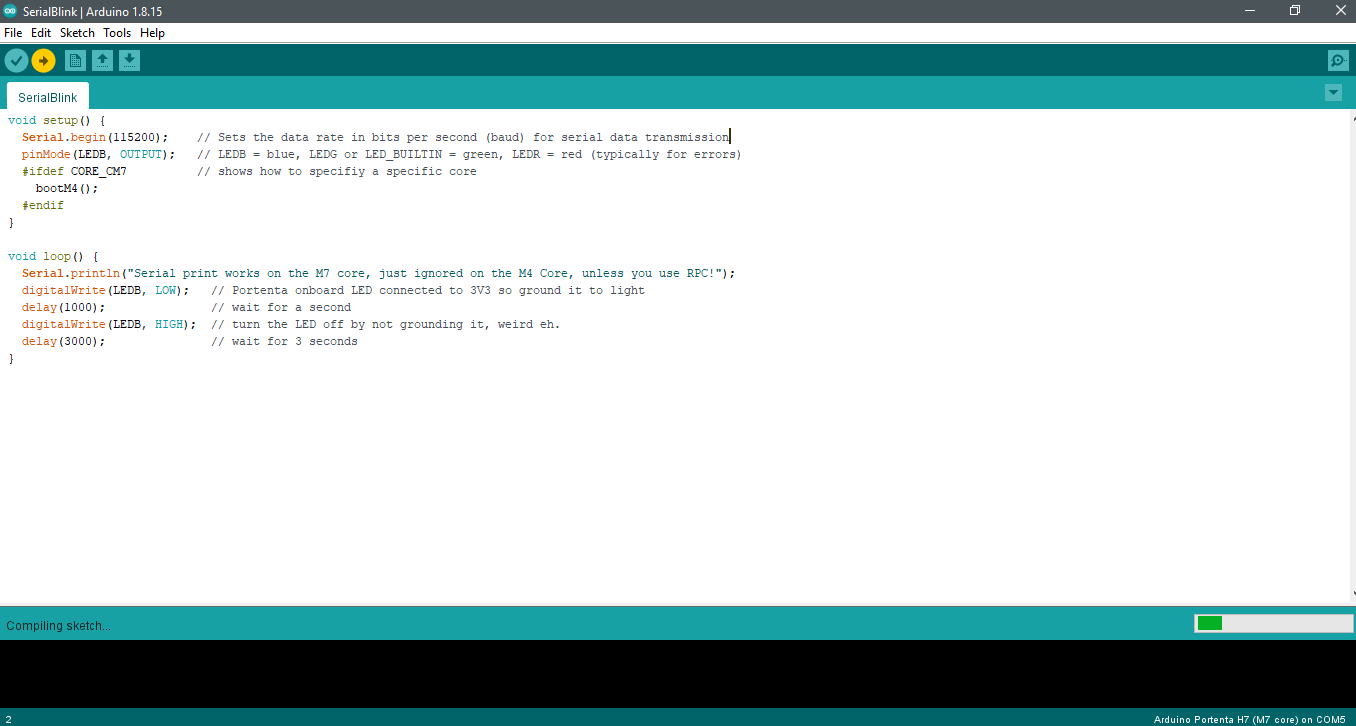
\includegraphics[width=0.8\textwidth]{Arduino/SerialBlinkM7}
	\caption{Serial Blink Sketch}
	\label{figure 5.5}
\end{figure}

In order to use core M4, we need to de-select the core M7 from the board and select core M4.After selecting, we can see at the bottom the selected core for confirmation. Also, We need to write another sketch and  now change the LED color to red in the sketch and add a delay of 4 seconds. 
\begin{figure}[H]
	\centering
	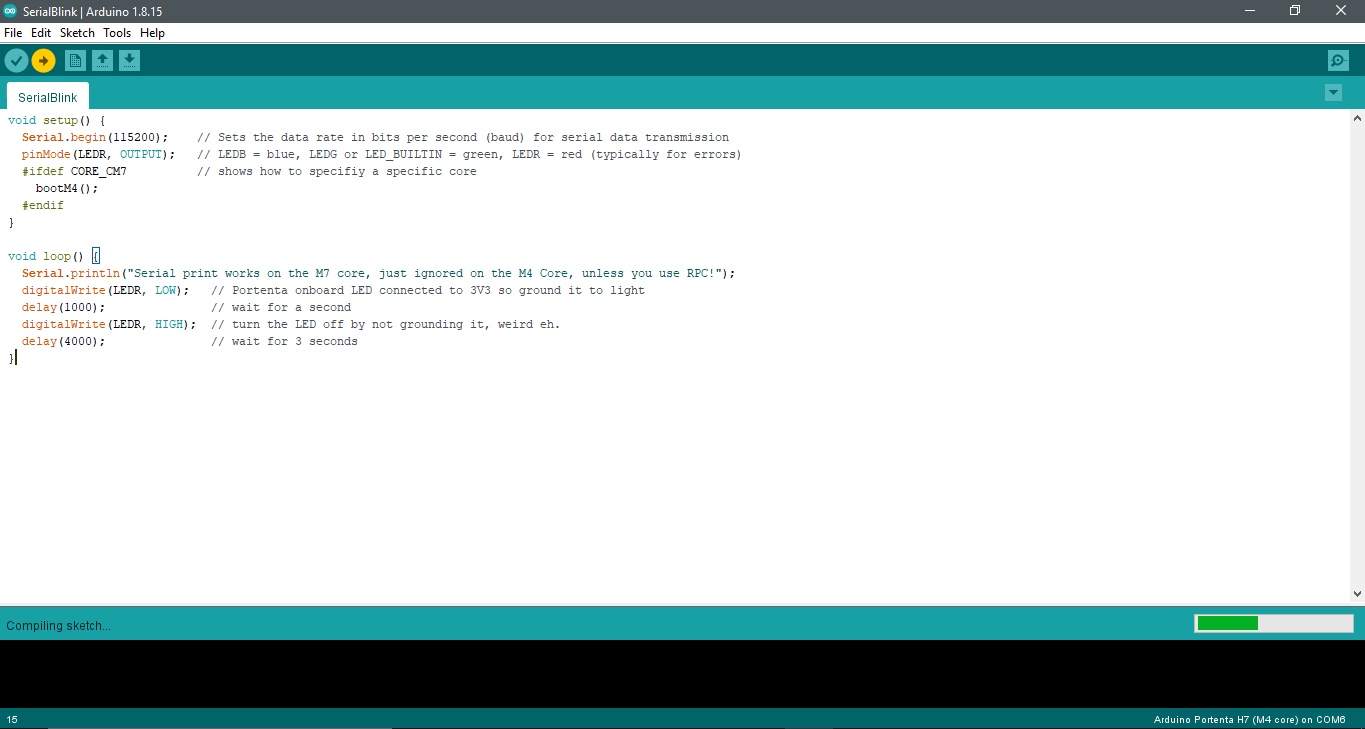
\includegraphics[width=0.8\textwidth]{Arduino/SerialBlinkM4}
	\caption{Serial Blink Sketch}
	\label{figure 5.6}
\end{figure}

Notice that in the output both LED blue and green blinks and at a point in time they almost blink together resulting in a Lila color. This shows the dual core processing concept by using an LED.

\begin{figure}[H]
	\centering
	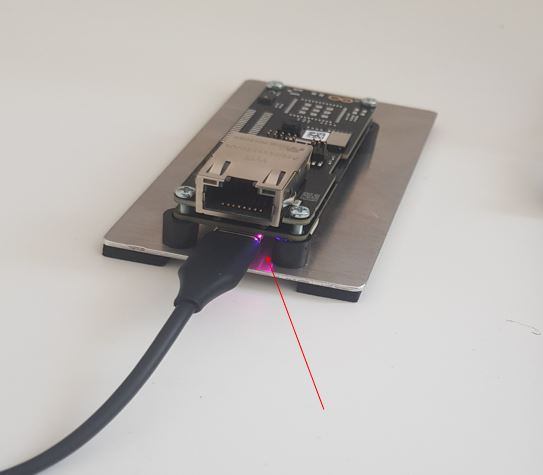
\includegraphics[width=0.8\textwidth]{Arduino/outLedlia}
	\caption{Output LED color}
	\label{figure 5.7}
\end{figure}
It can be seen from the figure \ref{figure 5.7} that the output LED blinks in lila color due to the overlapping of the green and blue LED blinking at the same time.
\chapter{First Steps with the Vision Shield}
\section{Introduction}
In this chapter we will be going through the installation of OpenMV IDE and the steps required for connecting the Arduino Portenta H7 with the Vision Shield using the OpenMV IDE. Further, we will be looking at the overview of the OpenMV IDE and what are the tools provided in the IDE.  Finally, we will be implementing some of the example programs provided in the OpenMV IDE.
\section{Update Bootloader version}
The OpenMV IDE is a premier integrated development environment which is a software tool  to use the openMV camera present on the Arduino vision shield.  It has a text editor ,frame buffer viewer with a histogram display and a debug terminal. It can be used across platforms, supporting Windows, Mac OS, Linux and Raspian. It was built for machine vision applications and is programmed in python\cite{OpenMV:2021}.
Now we need to connect our Arduino Portenta board with the vision shield. To do this, first we need to update the bootloader version using the PortentaH7\_updateBootloader sketch in the examples from the arduino IDE\cite{Romero:2020a}. After connecting the Arduino Vision shield with Arduino Portenta H7 board and plugging in to the laptop , go to the Arduino IDE and select examples and click on Portenta system and then select PortentaH7\_updateBootloader.
\begin{figure}[H]
	\centering
	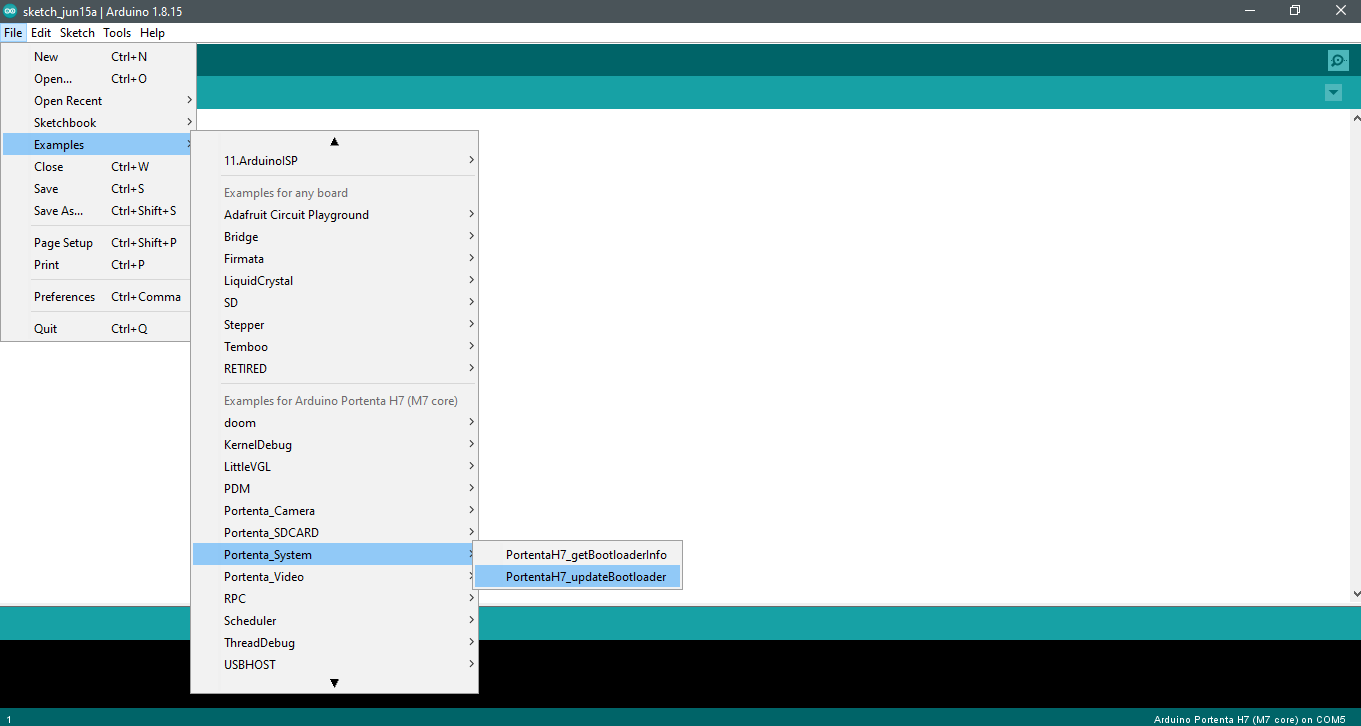
\includegraphics[width=0.8\textwidth]{Arduino/updatebootloader}
	\caption{Update Bootloader}
	\label{figure 6.1}
\end{figure}
Then run this sketch by selecting the right port.
\begin{figure}[H]
	\centering
	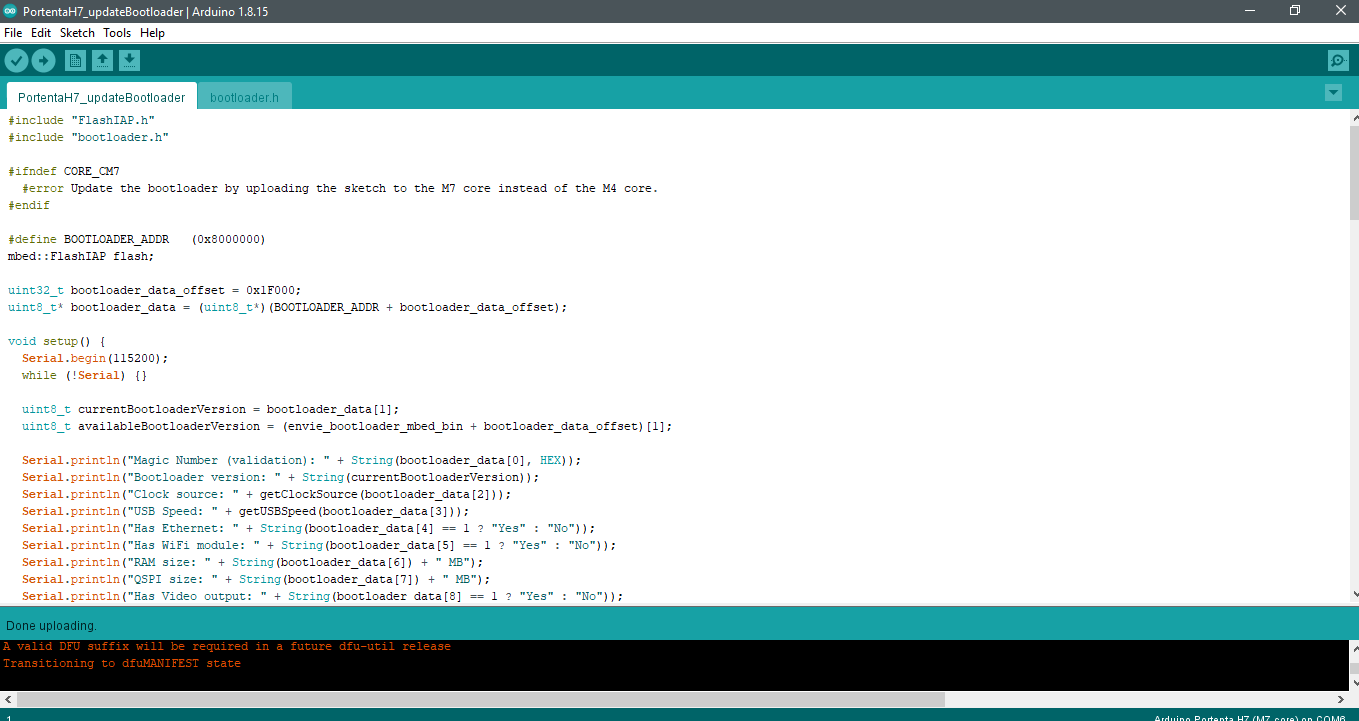
\includegraphics[width=0.8\textwidth]{Arduino/uploadBootloadersketch}
	\caption{Updload Bootloader sketch}
	\label{figure 6.2}
\end{figure}
After the upload is done, go to Tools and click on Serial monitor. A dialog box opens asking to update the bootloader version. Then press 'y' and enter. Now the bootloader version is updated.
\begin{figure}[H]
	\centering
	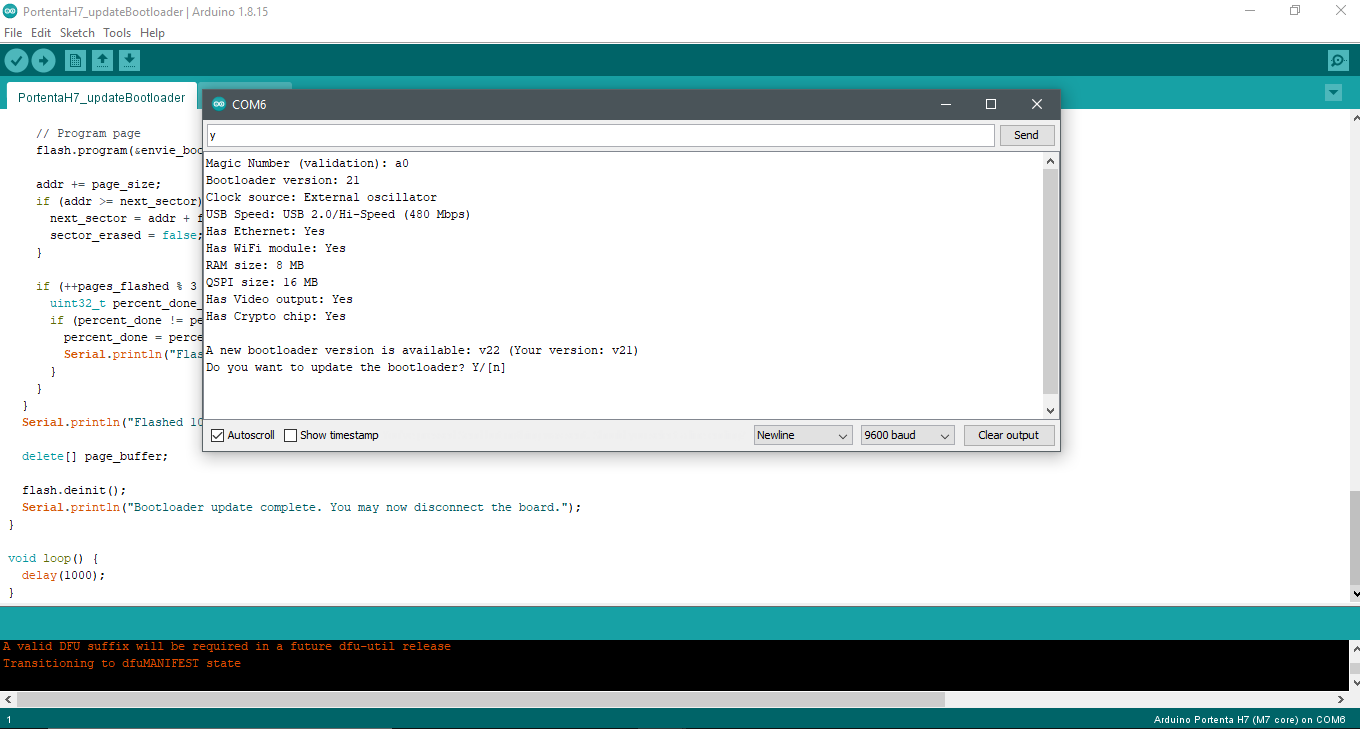
\includegraphics[width=0.8\textwidth]{Arduino/updatingootloader}
	\caption{Updating Bootloader}
	\label{figure 6.3}
\end{figure}

\section{OpenMV Examples}

\subsection{Creating a basic face filter with OpenMV}
In this example we use a smiley image in portable bitmap image(.pbm) format because OpenMV supports bmp, pgm or ppm image formats and not the other image formats such as .png \cite{Romero:2020}.  This image will be overlayed on the face when it detects a face in the camera stream. 
Download the image and copy it into the flash drive.
First we load the image into a variable named as faceImage using the Image() function. We use copy\_to\_fb to false because we don?t want it to be copied automatically in to the frame buffer. Next we calculate the scale ratio to scale the bitmap image to match the detected face in the camera stream using the function \PYTHON{scale\_ratio=faceWidth/faceImage.width()}
Then we draw the bitmap image on the detected face using the function \PYTHON{draw\_image()}.
Here the face detection is done using the Haar cascade algorithm. In this algorithm, it has multiple stages in which the output of one stage gives additional information  to the input of next stage in the cascade. By doing this, it calculates the edges, lines, contrast checks in different stages and ultimately detects the face and draws a bounding box around it. 


\begin{figure}[H]
	\centering
	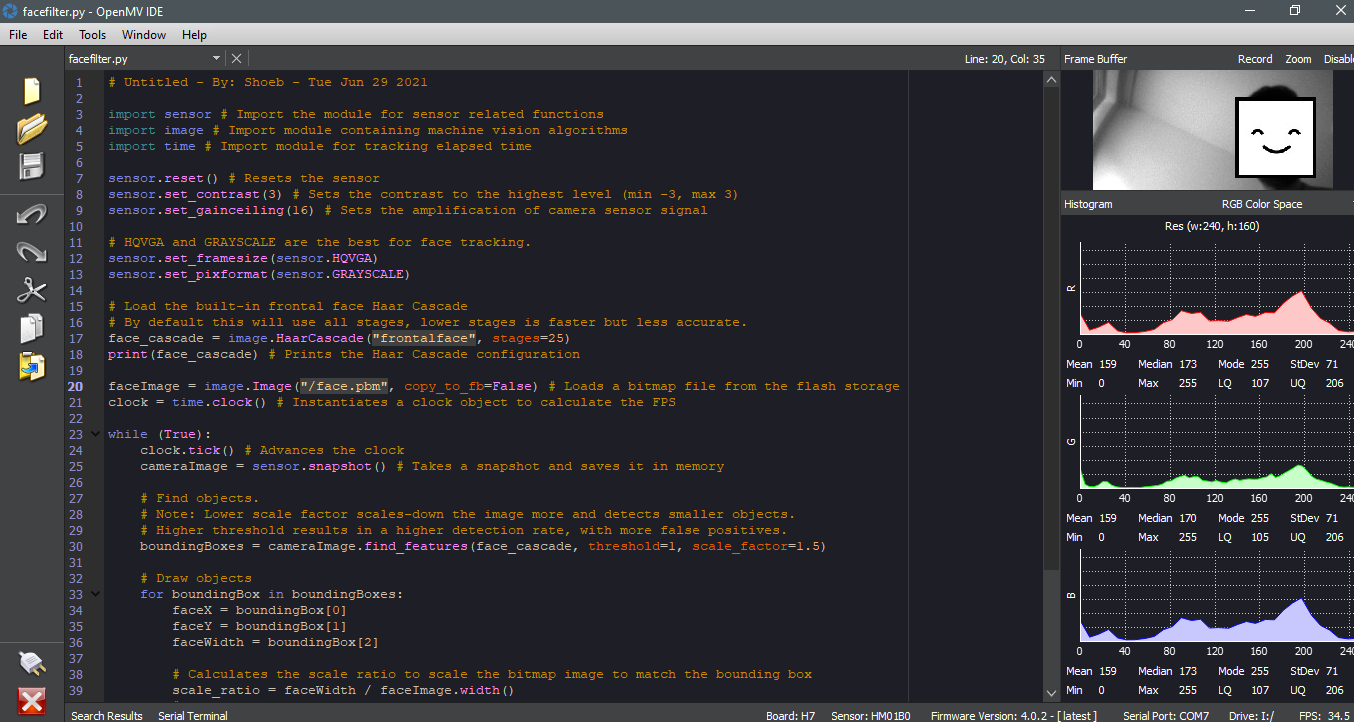
\includegraphics[width=\textwidth]{Arduino/facefilter}
	\caption{Face Filter output}
	\label{figure 6.10}
\end{figure}
As we can see from the above figure  \ref{figure 6.10} that as soon as a face is detected in the camera stream, the bitmap image which was loaded earlier is overlapped on to the detected face.
\subsection{Face tracking }
In this example, we are going to detect face and draw a bounding box around it. It uses the Haar cascade algorithm to detect faces.To do this, go to files in the OpenMV IDE and open examples and select face\_tracking. In the program, firstly, we  reset the sensor using \PYTHON{sensor.reset()} function and we  set the frame size to QVGA and set the pixel format to grayscale. Next we  load the Haar cascade using the function \PYTHON{image.HaarCascade()} . Next we  use the keypoints feature of OpenMV camera to track a face after it is detected by Haar cascade algorithm. For this, first we set the keypoints to none and when the face is detected we will use the function \PYTHON{image.find\_keypoints()} function. Then by using \PYTHON{draw\_rectangle()} function we draw a rectangle around the detected face and draw keypoints using \PYTHON{draw\_keypoints()} function. After this, we extract keypoints in the whole frame and then match this keypoints with first keypoints which was used only for face using \PYTHON{image.match\_descriptor()} function If the keypoints match is greater than 5 then we draw a rectangle around the matched feature.
\begin{figure}[H]
	\centering
	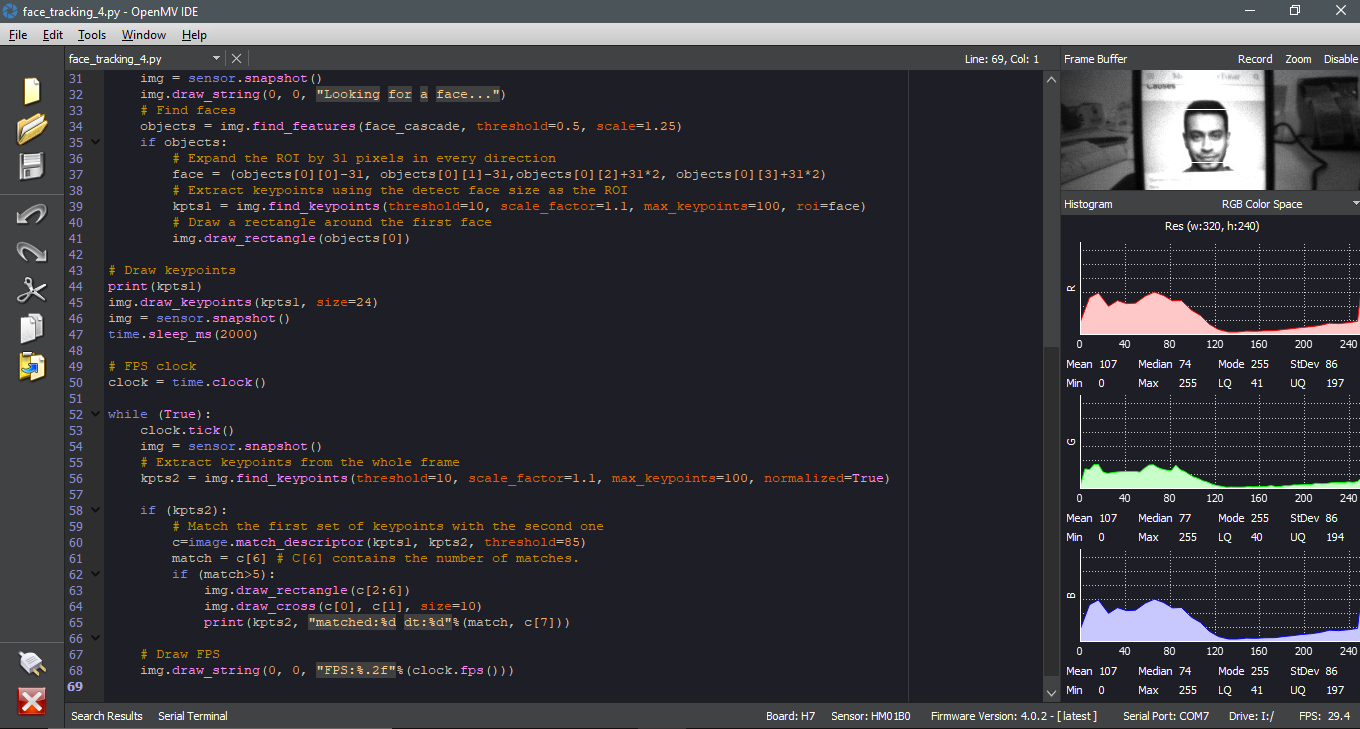
\includegraphics[width=\textwidth]{Arduino/face_tracking}
	\caption{Face tracking output}
	\label{figure 6.11}
\end{figure}
After we run this sketch, we need to point the vision shield camera towards a face and focus it properly. As soon as the face is detected in the camera stream , a rectangular box is formed around it indicating the detected face in the image. In this example, we can see that it clearly identifies the face and the bounding box is also generated around it.
\subsection{Finding circles around the objects}
In this example, we find the circles in an image using Hough transform algorithm. This algorithm is used in image processing for extracting the features such as circles or ellipses in an image.  For programming this,  we first reset the sensor as described in earlier examples. Then we take snapshot from the camera stream using \PYTHON{sensor.snapshot()} function. Then we find the circle in the image using  \PYTHON{find\_circles()} function. Lastly  we draw circles using \PYTHON{draw\_circles()} function.
\begin{figure}[H]
	\centering
	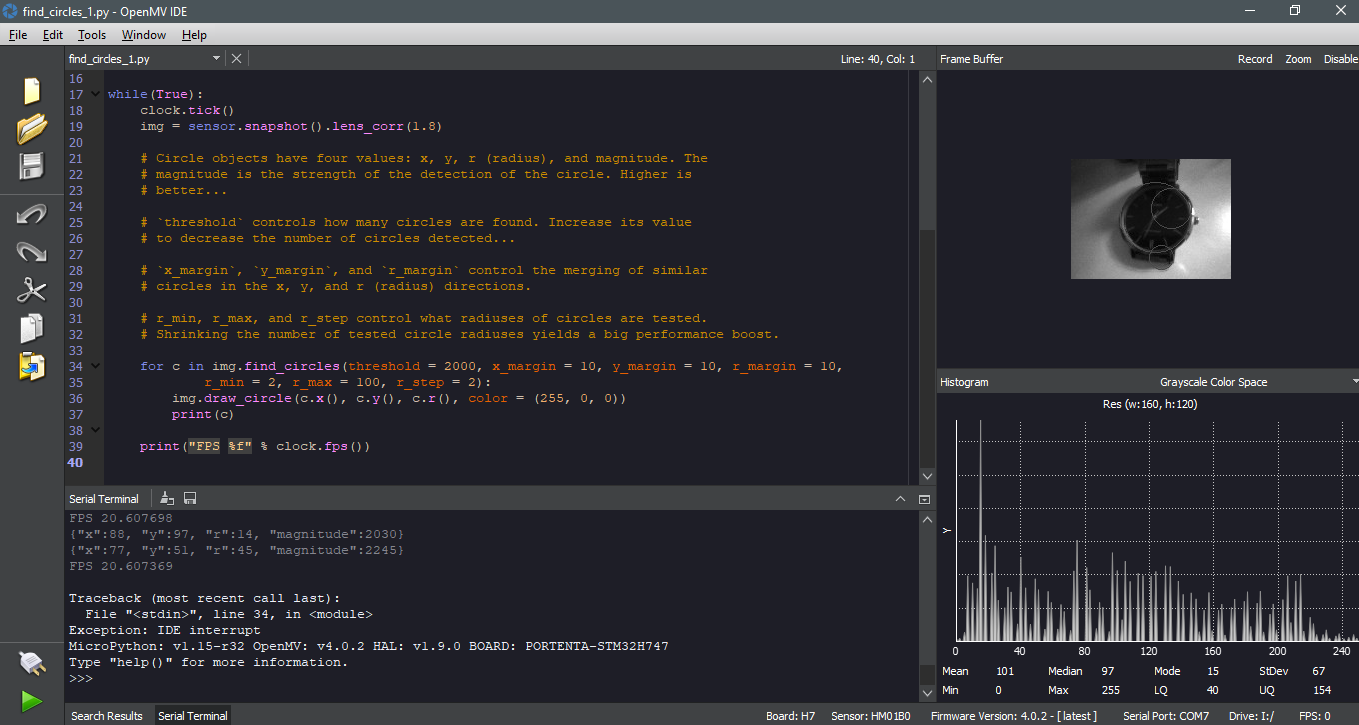
\includegraphics[width=\textwidth]{Arduino/find_circles}
	\caption{Find circles output}
	\label{figure 6.12}
\end{figure}
As can be seen from the figure \ref{figure 6.12},the ouput shows that the circles are drawn on the border of the watch. we need to bring the objects closer to the camera so that the focus is set properly in order to detect the circles around the objects.  
\subsection{QR Code information extraction}
In this example we extract the information from QR code by using the vision shield.  This is an interesting feature of the openMV camera present in the vision shield. In order to program this, we first follow the same initialization steps as mentioned in the earlier examples.  We then take a snapshot from the camera stream using the sensor.snapshot() function and then we do the lens correction to 1.8 in order to get a better quality image using \PYTHON{lens\_corr()} function.  To extract the QR code we use \PYTHON{find\_qrcodes()} function and then we draw a rectangle around the QR code using \PYTHON{draw\_rectangle()} function.
\begin{figure}[H]
	\centering
	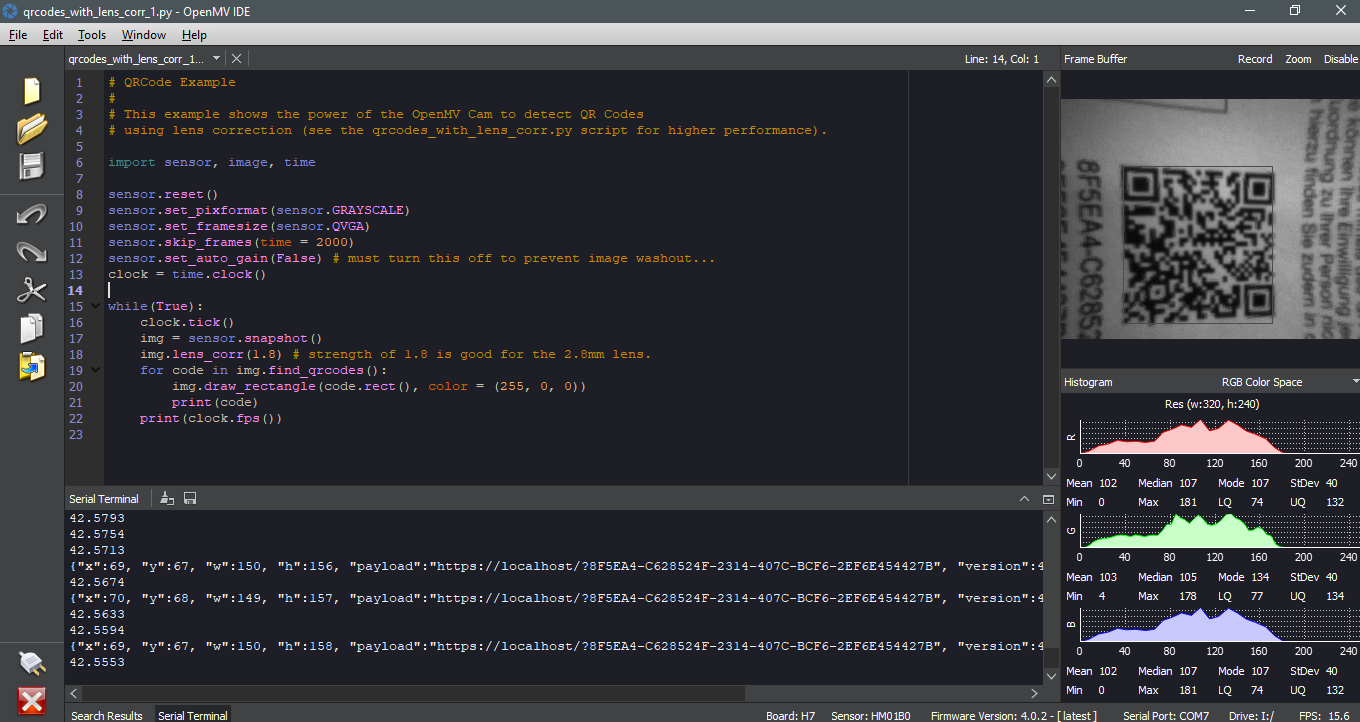
\includegraphics[width=\textwidth]{Arduino/QRcodedetection}
	\caption{QR Code output}
	\label{figure 6.13}
\end{figure}
In the output figure \ref{figure 6.13} we can see that a rectangular box is created around the QR Code and the information is extracted from it and it can be seen in the output serial terminal.








\chapter{MicroPython \& OpenMV}
\section{Introduction}
In this chapter we will be looking at MicroPython and OpenMV in detail. We will be describing some of the features of the MicroPython programming language and how we can run MicroPython scripts on the Arduino Portenta H7 board by using the OpenMV IDE. We will be implementing a basic MicroPython script in the OpenMV IDE to blink LED's on the Arduino Portenta H7 board.

\section{MicroPython}

MicroPython is a tiny Python programming language interpreter that works on small embedded development boards and is open source. Instead of using complex  low-level languages like C or C++, MicroPython allows us  to write clean and simple  Python code to control hardware (what Arduino uses for programming). It is a lean and efficient Python 3 implementation that includes only a tiny part of the Python standard library and is optimized for use on microcontrollers and in constrained environments and it is compact enough to fit and run within just 256k of code space and 16k of RAM.\cite{Romero:2020a}
It has unique features which makes it different from other embedded systems such as :
\begin{itemize}
	\item \textbf{Interactive REPL(Read-Evaluate-Print-Loop)} :  This helps in connecting to a board and execute the code without any need for compiling or uploading. It is a four step process in which it first reads the user input, evaluate the code, print any results and loop back to first step.
	\item \textbf{Extensive software library} : MicroPython like the normal python programming language has libraries built in to support many tasks. For example parsing JSON data from a web service, searching text with a regular expression, or even doing network socket programming is easy with built-in libraries for MicroPython.
	\item \textbf{Extensibility} : MicroPython is extensible with low-level C/C++ functions which means we can combine high level MicroPython code with faster low level code when needed.
\end{itemize}
The MicroPython programming language implements the core python 3 language but it can?t implement the entire standard library of Python 3 because trying to fit big libraries into tiny boards with just kilobytes of memory is not possible. One thing to note is that MicroPython is only a programming language interpreter whereas Arduino is an entire ecosystem which has the Arduino IDE and the hardware which in this case is Arduino Portenta H7.

\section{Implementing MicroPython on Portenta H7 with OpenMV IDE}
MicroPython scripts can be run on the Arduino Portenta H7 with the help of OpenMV IDE\cite{Romero:2020}. OpenMV comes with it?s own firmware which is built on MicroPython. We can explore the features of the Arduino Portenta H7 by using different classes and modules provided in MicroPython.

In order to implement MicroPython on the Arduino Portenta H7, we first need to connect the Arduino Portenta H7 with the computer using a USB -C cable and flash it by double pressing the reset button. After the flashing is done the bootloader gets updated while flashing the green LED. Now we open the OpenMV IDE and click on connect option provided at the bottom of the screen as done in the earlier chapters. This will install the latest OpenMV firmware to the Arduino Portenta H7 board. After the firmware is updated, we need to click on the play button to connect the board with OpenMV IDE and start programming in the IDE.
To be able to check whether MicroPython program can run on the Arduino Portenta H7 we write a simple program in MicroPython to blink LED?s on the board using the OpenMV IDE.
\subsection{Example script for blinking builtin LED on the Arduino Portenta H7 with OpenMV}
In the program we first import pyb module which contains board related functionality such as PIN handling. Then we create variables to control the built in LED?s using \PYTHON{pyb.LED()} function. Then we switch on the red,blue and green LED?s with a delay of 1000ms  using \PYTHON{redLED.on()} function and off the LED using  \PYTHON{redLED.off()}. Now after the program is complete we hit the play button in the bottom to upload the script.

\begin{lstlisting}
	import pyb
	redLED = pyb.LED(1) # built-in red LED
	greenLED = pyb.LED(2) # built-in green LED
	blueLED = pyb.LED(3) # built-in blue LED
	while True:
	# Turns on the red LED
	redLED.on()
	# Makes the script wait for 1 second (1000 miliseconds)
	pyb.delay(1000)
	# Turns off the red LED
	redLED.off()
	pyb.delay(1000)
	greenLED.on()
	pyb.delay(1000)
	greenLED.off()
	pyb.delay(1000)
	blueLED.on()
	pyb.delay(1000)
	blueLED.off()
	pyb.delay(1000)
\end{lstlisting}



We can see from the figure \ref{figure 7.2} that the output is flashing red,blue and green LED?s at a time interval of 1000ms. Therefore we can say that the MicroPython scripts can be run on the Arduino Portenta H7 with the use of OpenMV IDE
\begin{figure}[H]
	\centering
	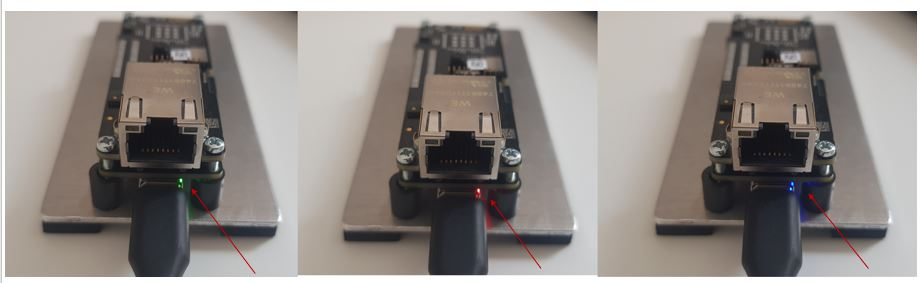
\includegraphics[width=\textwidth]{Arduino/outputmerged}
	\caption{Output RGB LED blinking red , blue and green}
	\label{figure 7.2}
\end{figure}



\chapter{First Application: Object Detection}

\section{What is Face Detection}
Face detection is Artificial Intelligence based computer technology which is used to detect human faces in images.
It determines the location and size of human faces in an image or video stream and after the face is detected it should return a bounding box on detected faces in it.It is considered as a quite challenging task in the field of computer vision because human face is a dynamic object and has great degree of variations in it. Face detection is used in many applications such as biometric security systems in which it is possible to track and monitor people in real-time.

There are two types of approches when detecting a face in an image, 1) Feature based approach 2) Image based aproach.

1) Feature-based approach : In this type of method the different features of the face  are found in the image for example detecting the eyes, nose eyebrows, mouth. As these features are consistent in an image which contains face despite other variabilities like lighting and poses. So the main idea behind this approach is to extract these features using edge detection techniques and based on these extracted features statistical models are built to describe the relationship and detect a presence of face in an image.
2) Image-based approach : The image based method try to learn templates from examples in images. That means this method relies on machine learning and statistical analysis techniques to find the facial charateristics to declare whether the image has face or no face present in it. In this method, neural networks are used for detection. 



\subsection{Challenges}
The challenges in face detections are the reasons for less accuracy and detection rates in images. Some of the challenges include :
\begin{itemize}
	\item Lighting Conditions : The lighting surrounding an image maybe low or high in parts of image which makes it difficult to detect faces.
	\item Distance : If the distance of the camera towards a face is very low or high then also it becomes difficult for detection.
	\item Orientation : The face orientation and angle to the camera can also cause detection failures.
	\item Complex background : If the background of the image contains more number of objects then it will become a difficult task for detection.
	\item Low resolution : If the image resolution is very low or the image contains noise then the accuracy of the detected face will be less.
\end{itemize}
\subsection{Solutions}
\begin{itemize}
	\item Optimal lighting conditions should be considered when tryin to detect a face in an image. A good evenly illuminated image helps in easy detection of face in an image.
	\item The distance between the camera and face should be optimum. In our case, a distance between 7cm-10cm is best suited for face detection.
	\item The number of training images with different angles and orientation should be taken to improve the detection rate in images with different orientations of faces.
	\item The background of the image should also be considered in such a way that the face which we are going to detect is not occluded because of more number of objects present in the image.
	\item Using state of the art methods like  convolutional neural networks(CNN) for face detection helps siginificantly in detection rate.
\end{itemize}
\subsection{Applications}
\begin{itemize}
	\item Quality Testing : Testing the quality of finished products in a production plant
	\item Surveillance : It is used for face detection in a crowd such as a public place or private place.
	\item Attendance : It can be used to detect the attendance of humans in a class and when combined with biometric security system it can also be used in access management in a building.
	\item Photography : Mobile phone cameras detect faces for autofocus in an image.
\end{itemize}
\chapter{Training a Custom Machine Learning Model for Portenta H7}

\section{Introduction}
In this chapter we are going to look at how to train a face detection model and what are all the steps required in training a model using the Edge Impulse platform. Further we will be looking at how to deploy the tflite model and implement in the OpenMV IDE the face detection model.

\section{How to train a face detection model }
Machine learning on microcontrollers is an interesting aspect as they can run on low power batteries for a long period of time. We can even put the microcontroller to sleep and only activate it when the camera or any other sensor notices an activity. The other interesting aspect is that machine learning models on a microcontroller can run without internet connection as they don't need to upload data to the cloud. Therefore the data is only present in the device which ensures data protection.\cite{Romero:2020}

\section{KDD Process}

\subsection{KDD Process for the object detection model}
Knowledge discovery in databases is the process of discovering useful knowledge from
a collection of unstructured or structured data. It involves different phases such as data selection,
preparation, timing data, mining, finding patterns, evaluation and verification. This process can be applied to the Edge Impulse platform in determining how the platform works in the background.
The process starts with a database consisting of images of objects which are to be trained in the model in order to be detected. Then a training dataset is prepared from the database and data processing is done before going for actual training. Then  the model is  trained, in this case using a Convultional Neural Network(CNN)  and the model is evaluated. Depending on the ouput the model is either fine tuned or changes in training dataset is made acordingly. This KDD process is described in detail for the face detection  model in the next sections.

\subsection{Database}
In order to train a machine learning model for face detection we first need to create a dataset of images consisting of faces.  We can do this by capturing the images using the Vision Shield camera. We can also download a dataset online and use it to train the model.  UTKFace  is one dataset with long age span(0 to 116 years old) consisting of over 20k single face images. We can download this dataset from the link \url{https://susanqq.github.io/UTKFace/}

\textbf{Selection of Dataset} : Manually captured images from the camera present on the Vision shield, UTKFace dataset.
\vspace{-1em}
\subsection{Add Dataset in the OpenMV IDE}
In order to add dataset in the OpenMV IDE, go to Tools then select Dataset Editor and click on New Dataset as shown in the figure \ref{figure 9.1}. Then select an empty folder in the drive where all the images will be stored. 

\begin{figure}
	\centering
	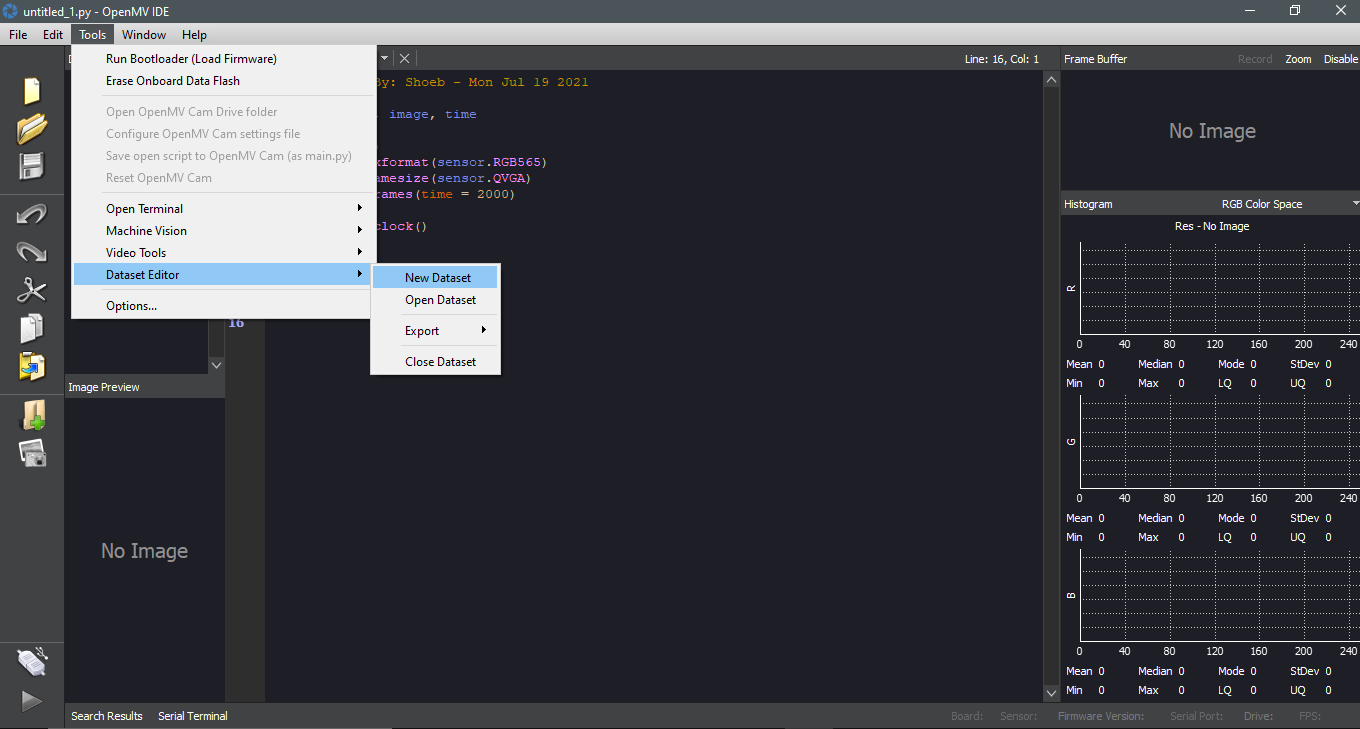
\includegraphics[width=\textwidth]{Arduino/AddDataset}
	\caption{Add Dataset}
	\label{figure 9.1}
\end{figure}

Then we defined two classes of images. Firstly,  we created face class and added images of face from the UTKFace dataset. Secondly, pen class is created by capturing pictures of pens of different types and at different positions using the Vision Shield directly from the OpenMV IDE. From the figure \ref{figure 9.2} we can see that two folders namely face.class and pens.class are created in the Dataset editor. We do this to help the model learn in distinguishing face from other objects, in this case a pen.

\begin{figure}
	\centering
	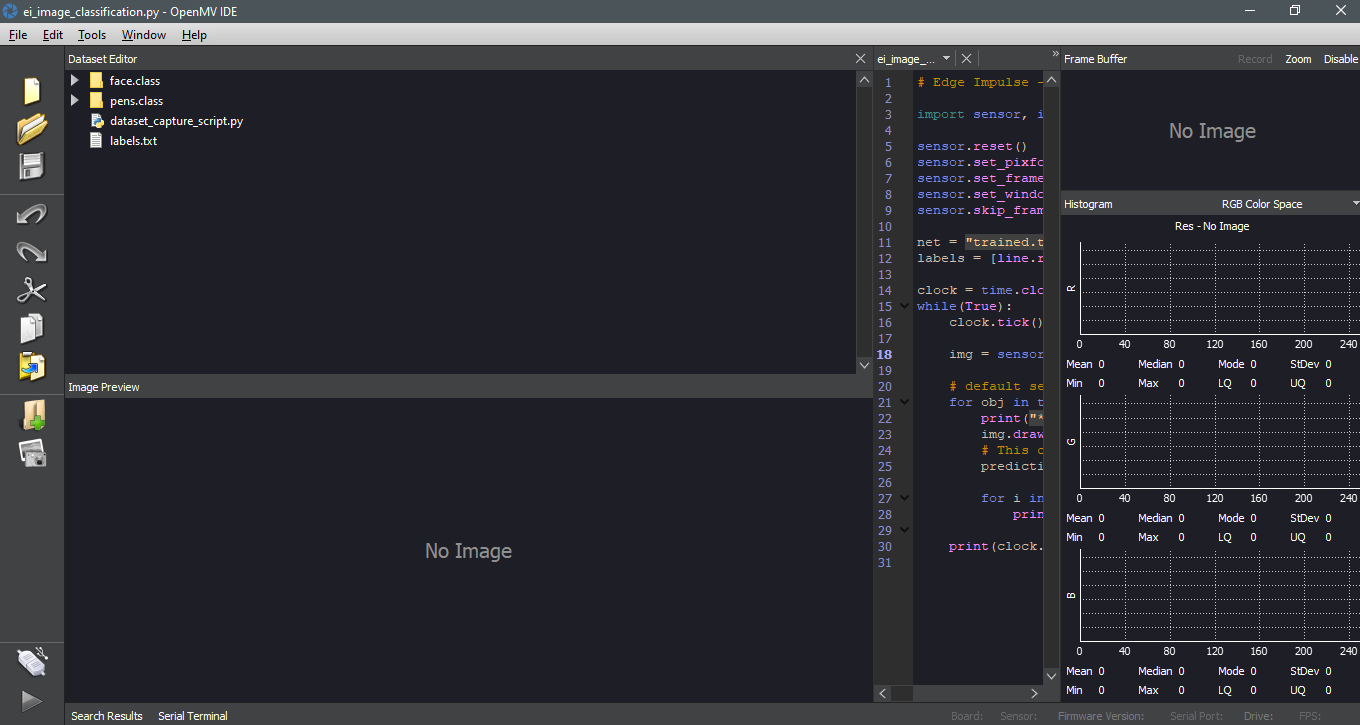
\includegraphics[width=\textwidth]{Arduino/Datasetclass}
	\caption{Dataset class Folders}
	\label{figure 9.2}
\end{figure}

Now that our dataset is prepared, we can now go for training the model. To do this,  we need to create a project in Edge Impulse platform. 

Firstly, we need to sign up / login in the Edge Impulse account by going to their webpage \url{https://www.edgeimpulse.com/} and create a new project named Face\_detector.


\subsection{Export the Data to Edge Impulse platform}

Now in the OpenMV IDE we need to export our data to the Edge Impulse website. To do this, click on Tools and then select Dataset Editor and then select Export and then select upload to Edge Impulse Project as shown in the figure \ref{figure 9.3}

\begin{figure}
	\centering
	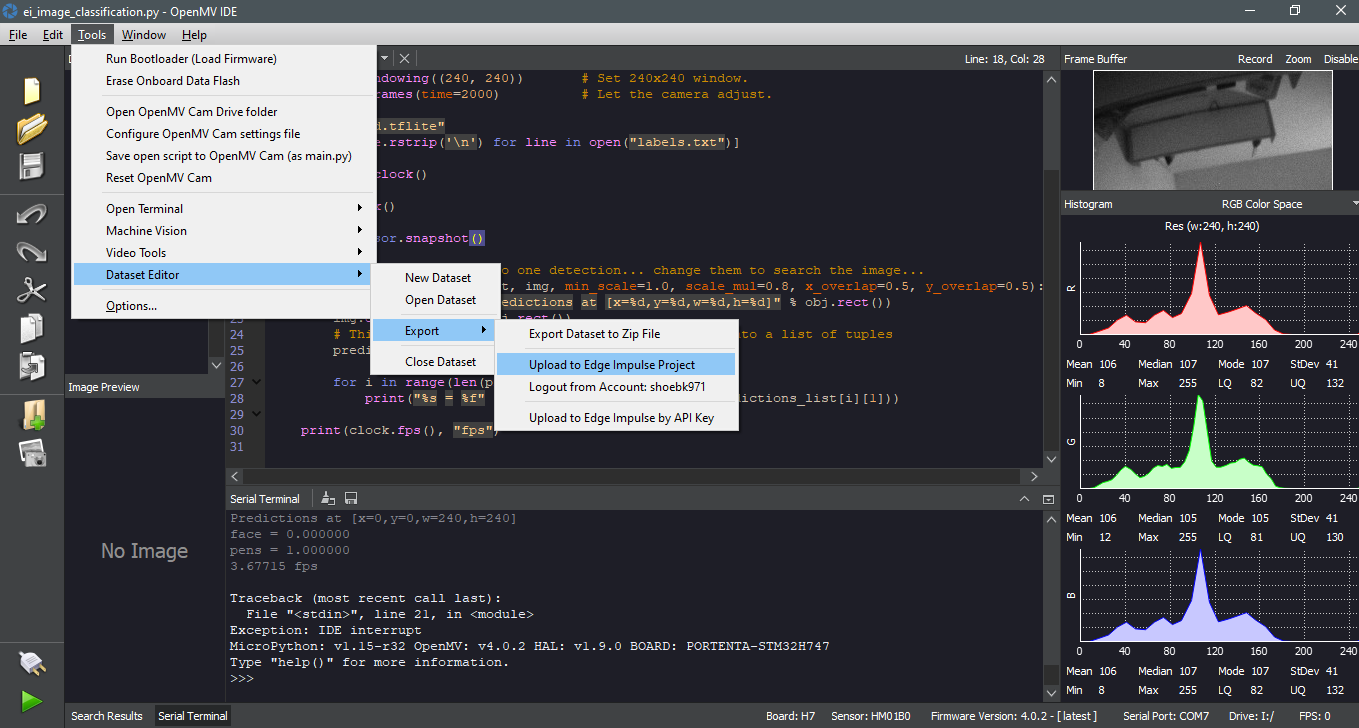
\includegraphics[width=\textwidth]{Arduino/exportedgeimpulse}
	\caption{export to Edge Impulse}
	\label{figure 9.3}
\end{figure}

\subsection{Data Selection}

Now go to the Edge Impulse website and click on data acquisition.  From the figure \ref{figure 9.4} we can see that all of our images with two labels have been exported from the OpenMV IDE to the Edge Impulse platform. It automatically divides the dataset in to training and testing data. Here it has divided into 487 items in training data and 51 items in testing data.

\begin{figure}
	\centering
	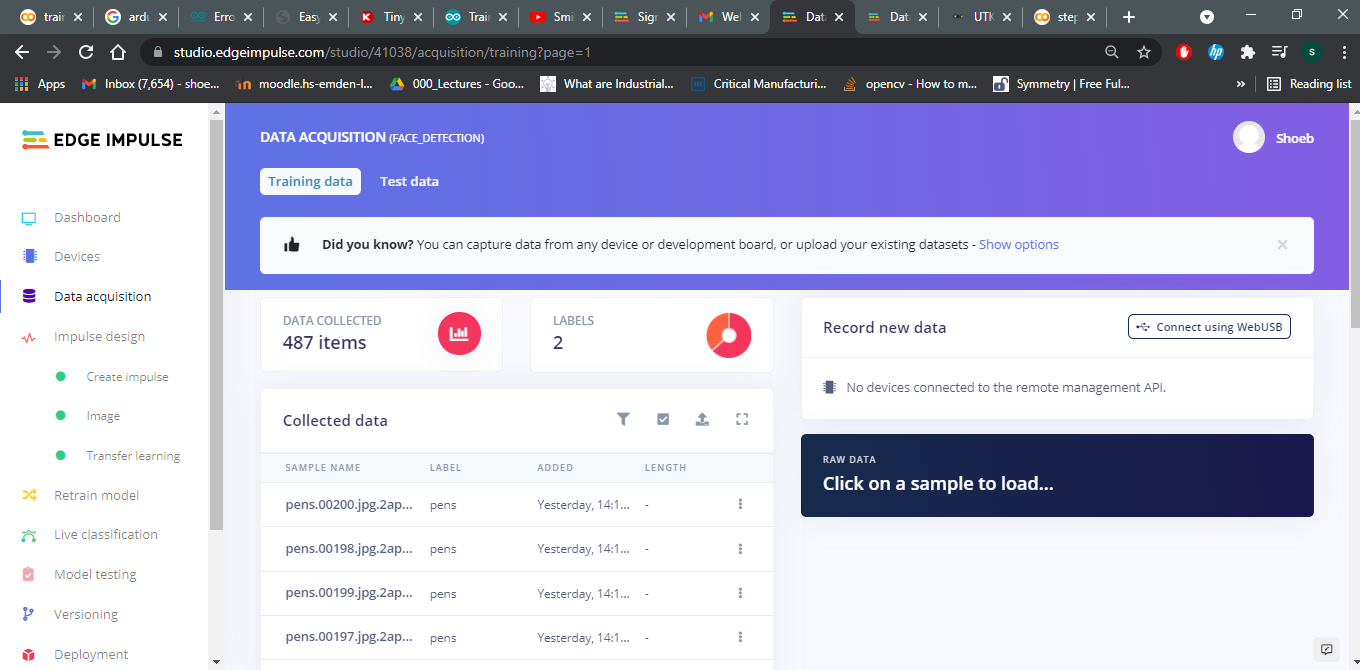
\includegraphics[width=\textwidth]{Arduino/DataAcquisition}
	\caption{Data Acquisition in Edge Impulse}
	\label{figure 9.4}
\end{figure}

\subsection{Data Transformation}
Now click on  Impulse design and set the image width and height in the Image data field, add processing block which is image in this case and apply transfer learning as shown in the figure \ref{figure 9.5}. After this, click on save impulse.

\begin{figure}
	\centering
	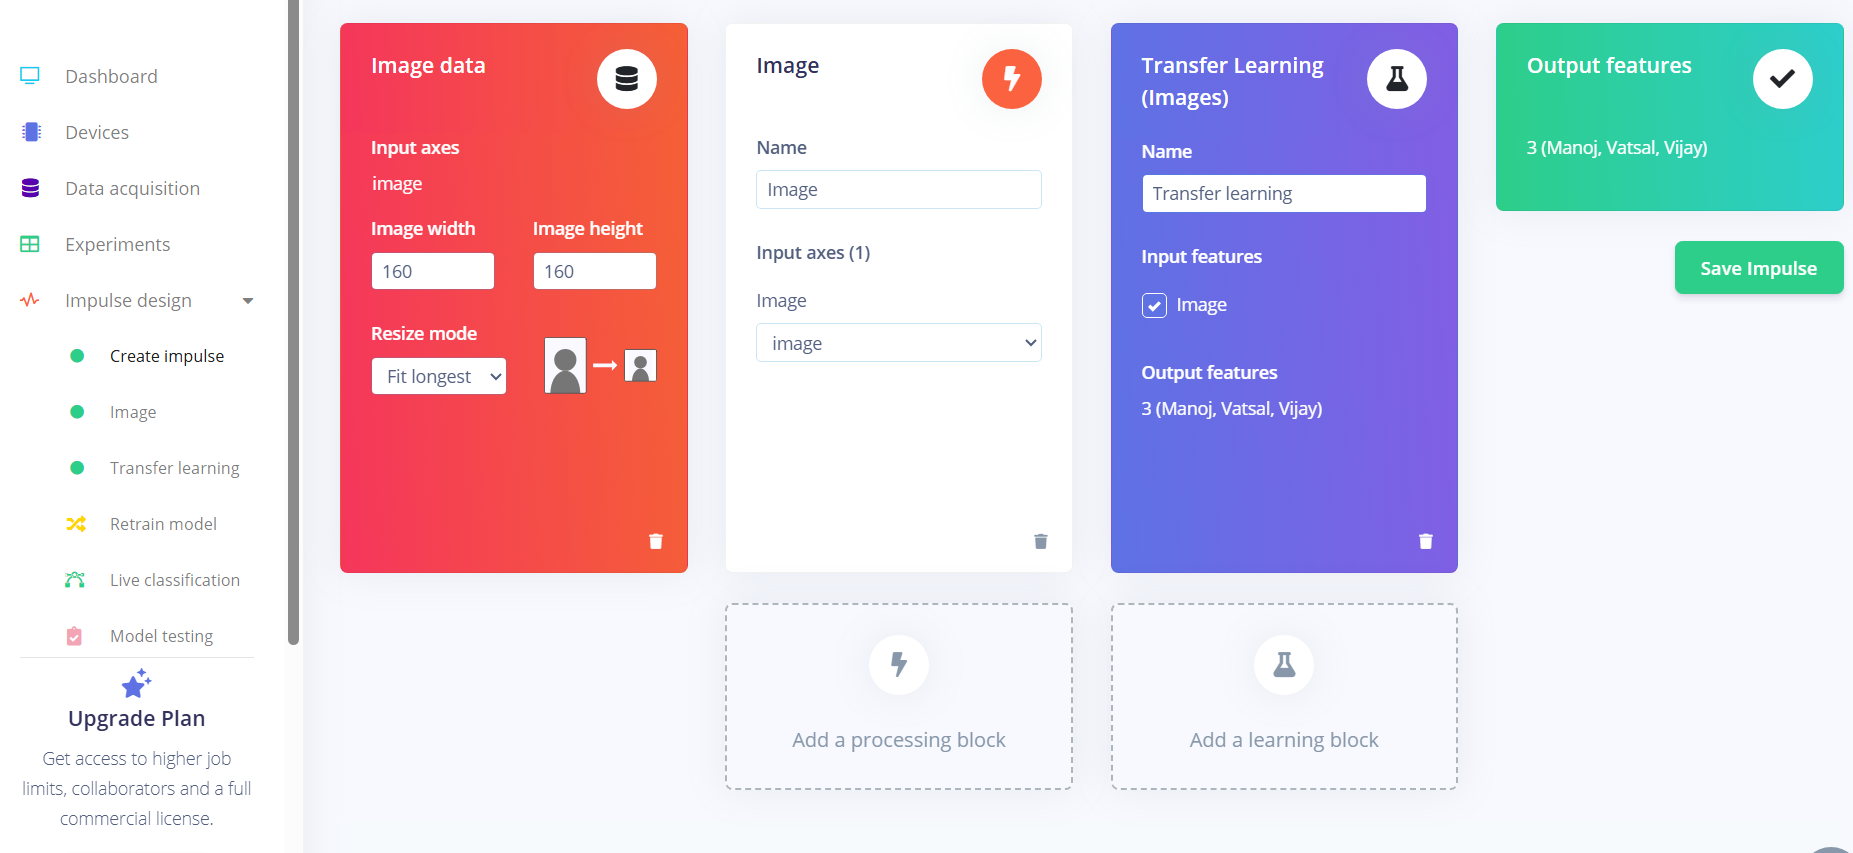
\includegraphics[width=\textwidth]{Arduino/ImpulseDesign}
	\caption{Impulse Design}
	\label{figure 9.5}
\end{figure}

Now click on Image tab on the left side of the screen and select the color depth to Grayscale and click on save parameters as shown in the figure \ref{figure 9.6}.

\begin{figure}
	\centering
	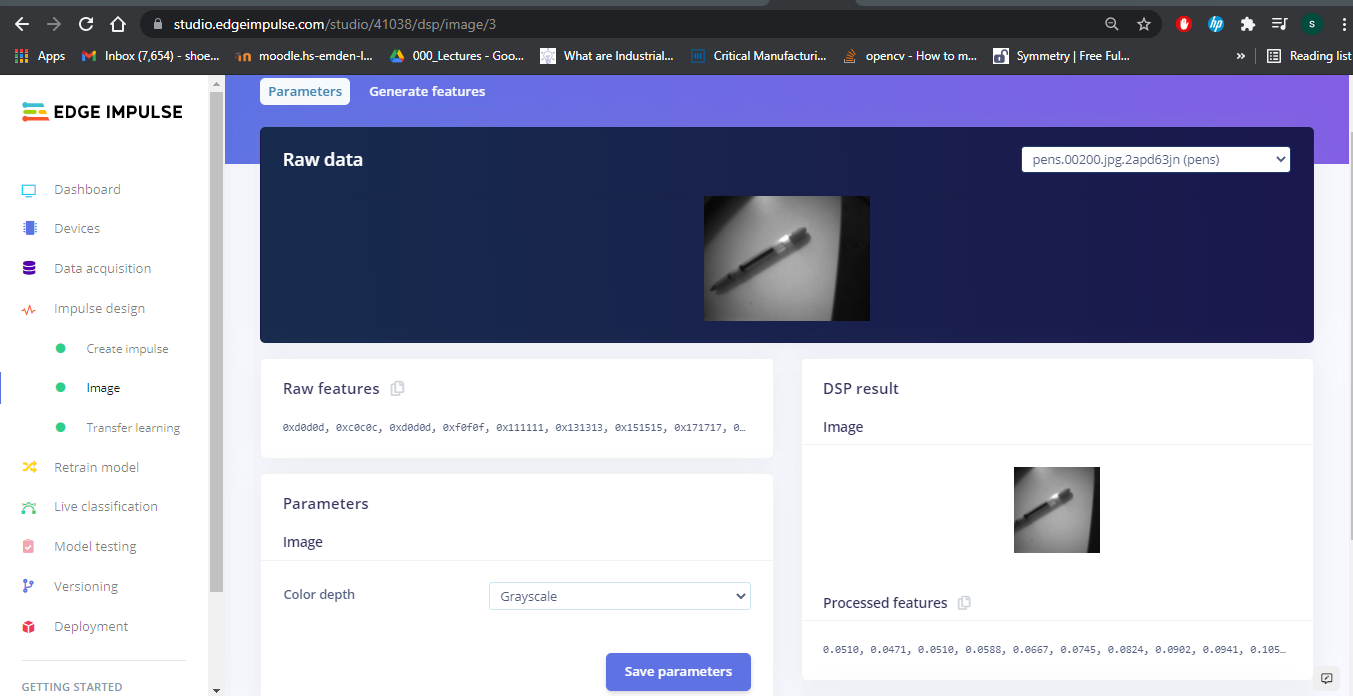
\includegraphics[width=\textwidth]{Arduino/Parameters}
	\caption{Save Parameters}
	\label{figure 9.6}
\end{figure}

Now click on Generate features and here we can see the number of items in the training dataset and number of classes as depicted in the figure \ref{figure 9.7}.  click on Generate features. 

\begin{figure}
	\centering
	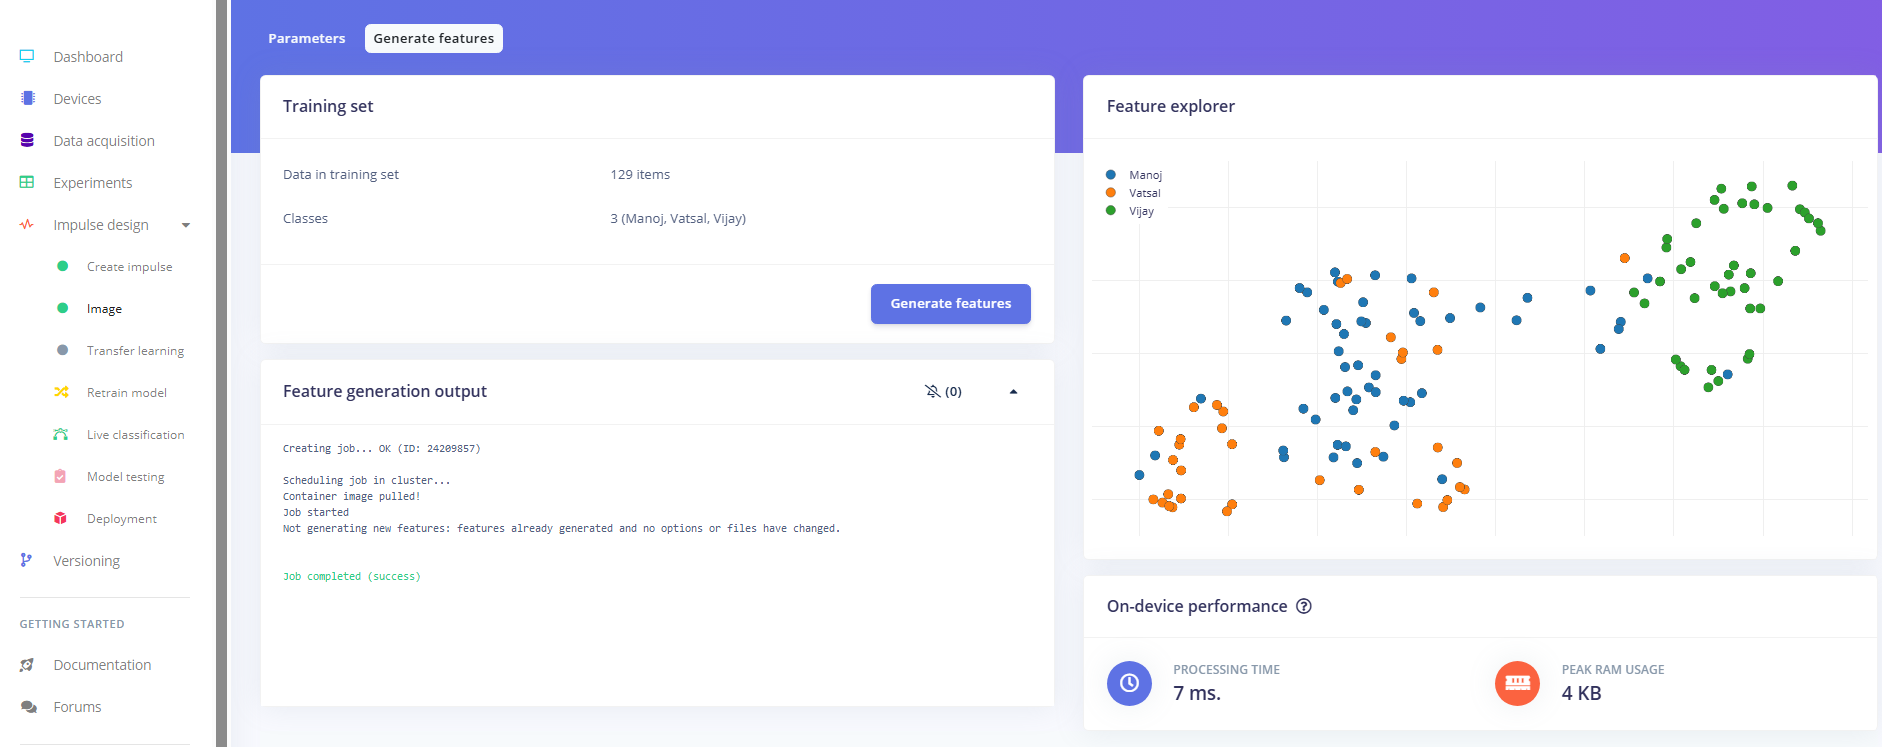
\includegraphics[width=\textwidth]{Arduino/GenerateFeatures}
	\caption{Generate Features}
	\label{figure 9.7}
\end{figure}

After the process is done we can see the feature explorer which contains the features of the dataset we have added and we can see that there is a clear difference between features of a face and a pen asshown in the figure \ref{figure 9.8}.

\begin{figure}
	\centering
	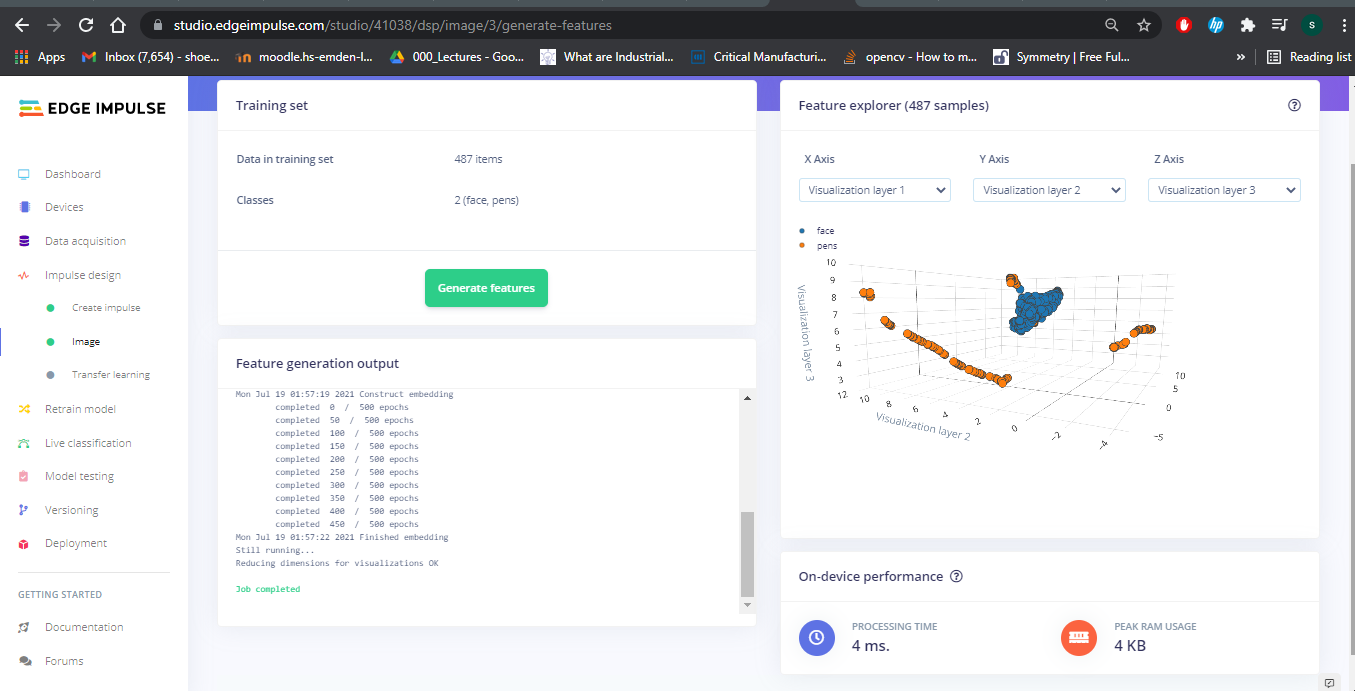
\includegraphics[width=\textwidth]{Arduino/FeatureExplorer}
	\caption{Feature Explorer }
	\label{figure 9.8}
\end{figure}

\subsection{Data training }

Now click on Transfer learning and select the number of training cycles which is epochs(50 in this case). Then we  select the architecture model for the convolutional neural network model which we chose MobilenetV2 here.
We can also edit the python script to train the model by clicking on neural network settings and selecting switch to Keras(expert) mode option as shown in figure \ref{figure 9.9}. The model uses Adam optimizer and Adadelta optimizer.

\begin{figure}
	\centering
	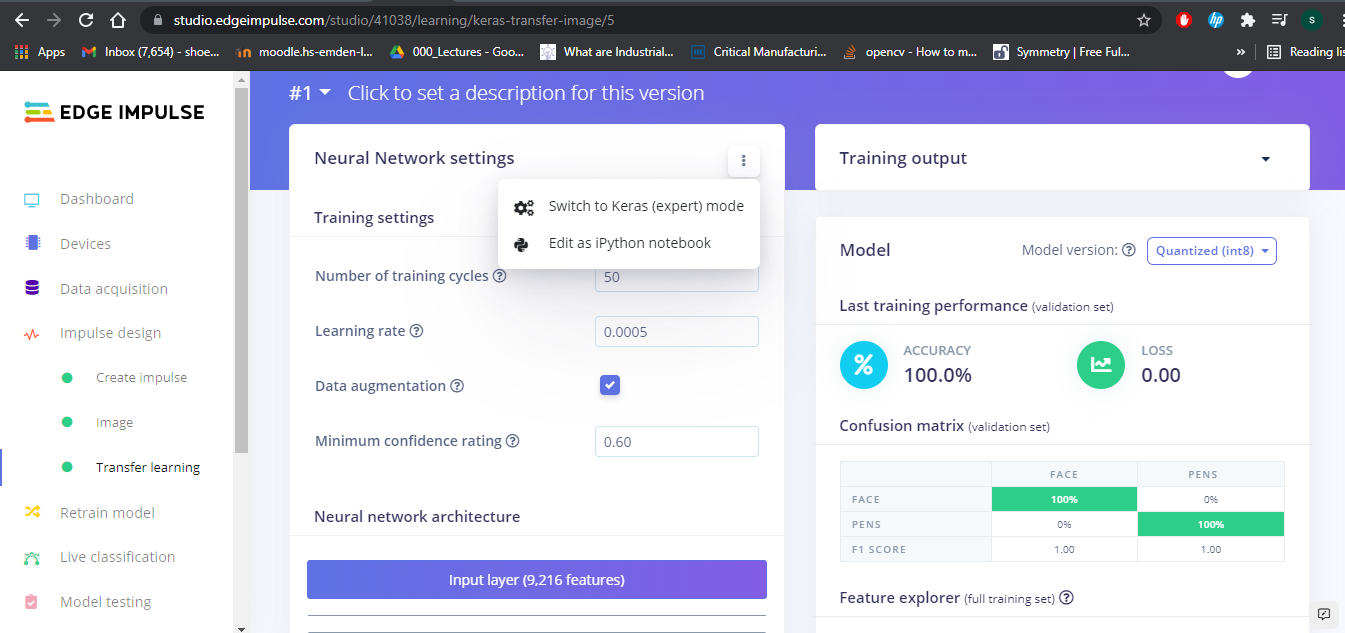
\includegraphics[width=\textwidth]{Arduino/EditProgram}
	\caption{Edit Neural Network Program }
	\label{figure 9.9}
\end{figure}

Now click on start training. After the training process is completed we can see the output accuracy  is 100\% and the loss percentage is 0 as shown in the figure \ref{figure 9.10}.

\begin{figure}
	\centering
	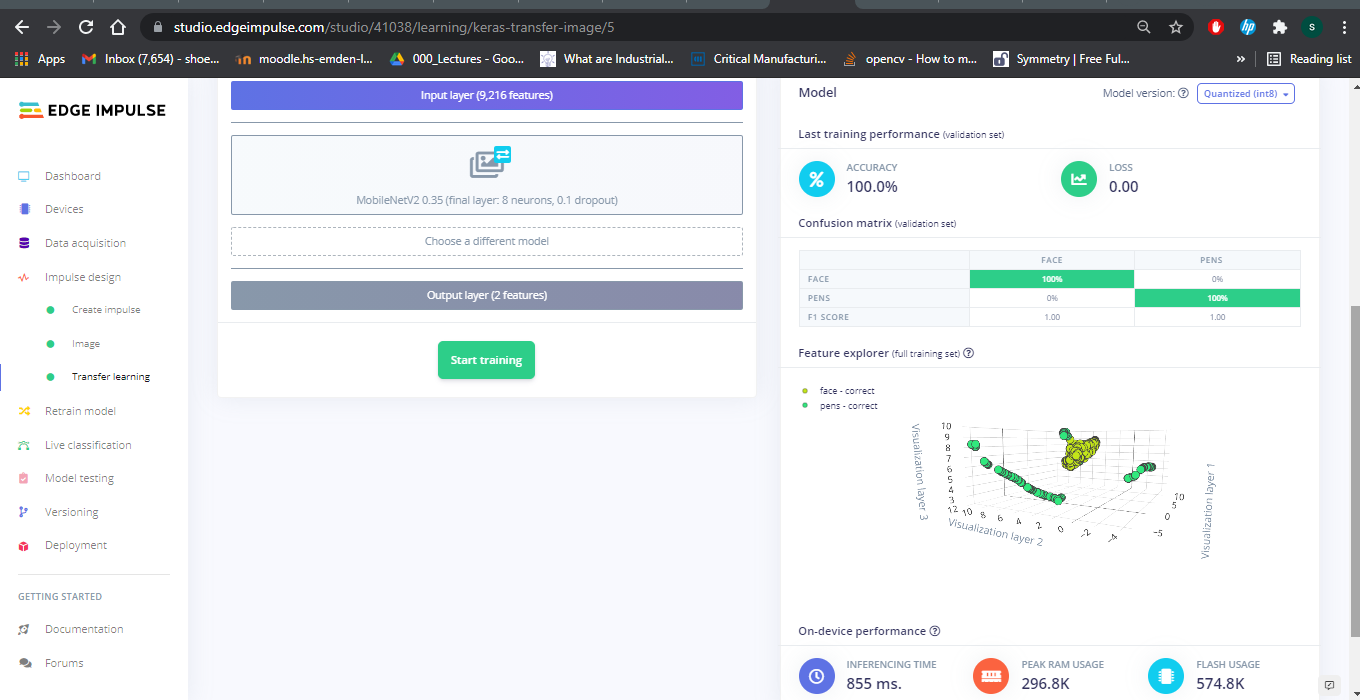
\includegraphics[width=\textwidth]{Arduino/Modeloutput}
	\caption{Model output }
	\label{figure 9.10}
\end{figure}

\subsection{Deploy to Arduino Porrtenta H7}
In order to deploy the trained model to the Arduino Portenta H7, we go to the Edge Impulse menu options and click on Deployment and then select OpenMV and click on Build as shown in the figure \ref{figure 9.11}. This will create a zip file which consists of TensorFlow Lite file named as trained.tflite and lables.txt along with the python script ei\_image\_classification.py. After downloading this we need to copy trained.tflite file and labels.txt file and paste it in the USB drive where our Arduino Portenta H7 is connected to the laptop.
\begin{figure}[H]
	\centering
	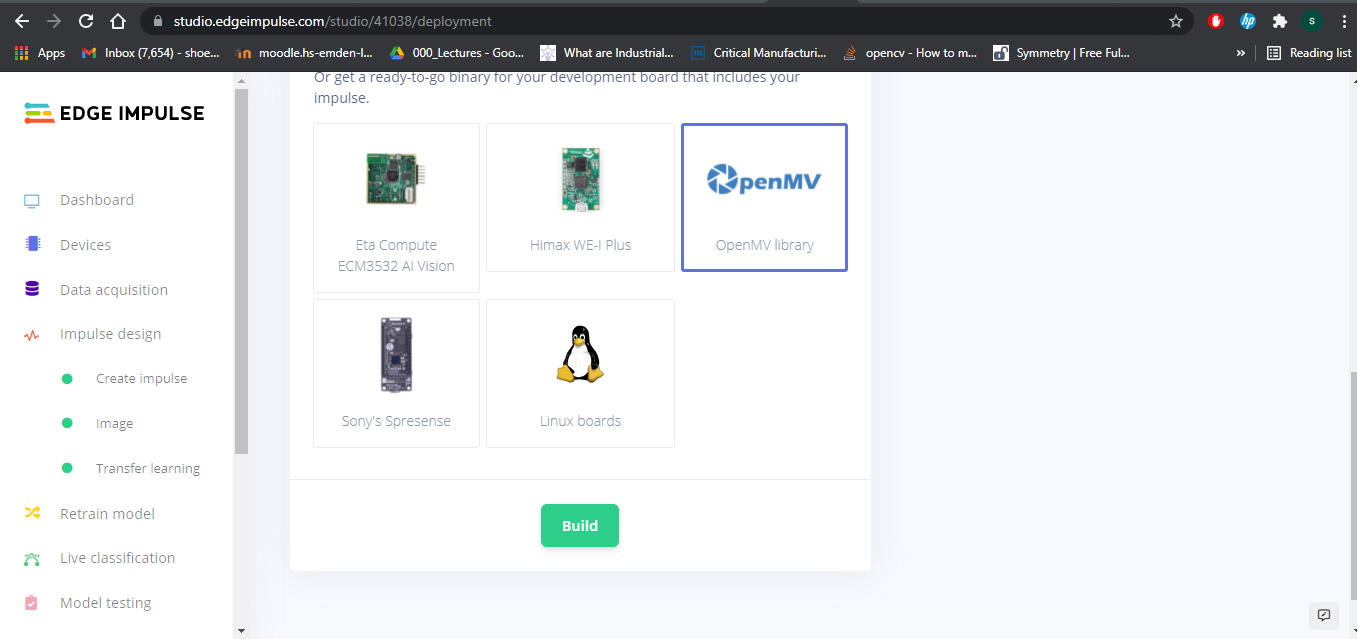
\includegraphics[width=\textwidth]{Arduino/Deployment}
	\caption{Deployment to the Arduino Portenta H7}
	\label{figure 9.11}
\end{figure}
\subsection{Testing the trained model using Vision shield and OpenMV IDE}
To test the trained model, we go to the OpenMV IDE and open the downloaded python script ei\_image\_classification.py and click on play button.Now move the vision shield towards the objects and open the serial terminal to see the output predictions. Here we can see from the figure \ref{figure 9.12} that the face is being detected and the prediciton is 1.0 which means it is 100\%

\begin{figure}[H]
	\centering
	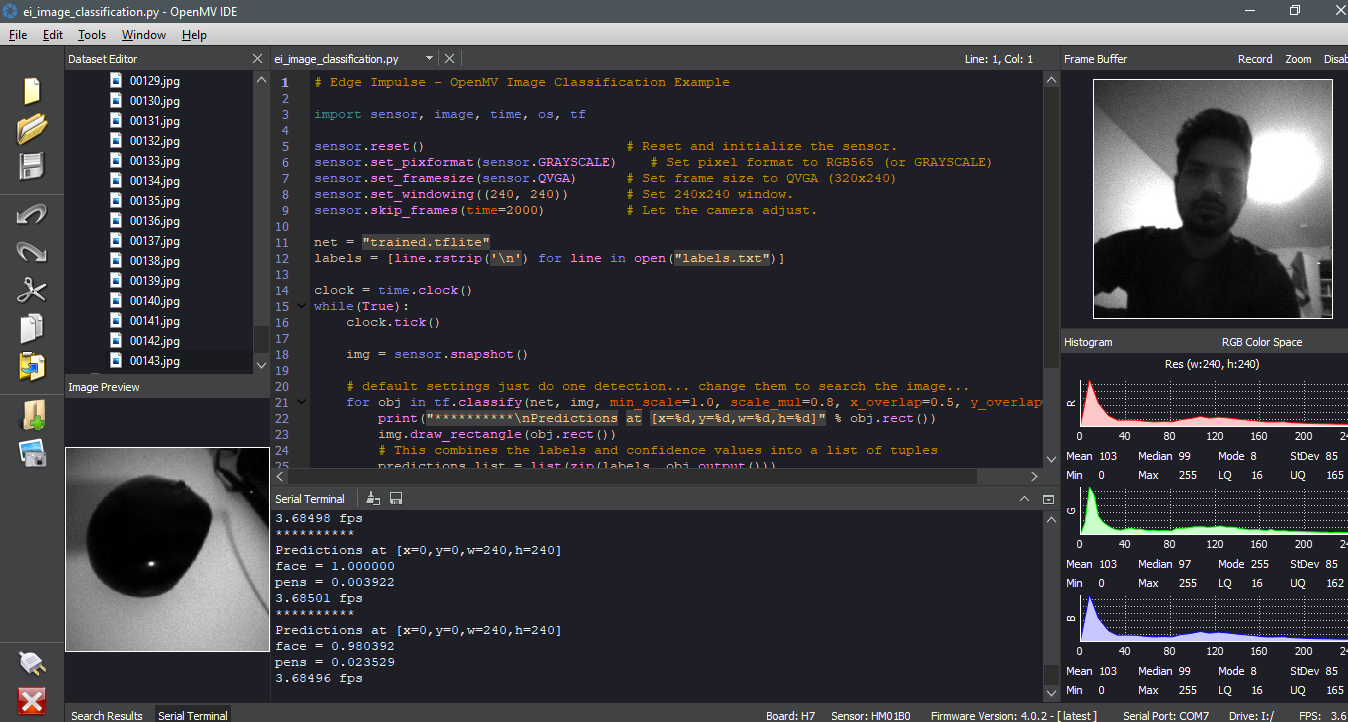
\includegraphics[width=\textwidth]{Arduino/Facedetetcted}
	\caption{Face detection output}
	\label{figure 9.12}
\end{figure}
In order to check whether the model differentiates between a face and other objects, we move the vision shield camera towards a pen and  we can see from the figure \ref{figure 9.13} that the face prediction is 0 and it predicts that the object is a pen at 0.96 which means 96\%. Therefore, we can say that the model is trained to be able to detect faces in an image or video stream captured by the Vision Shield.
\begin{figure}[H]
	\centering
	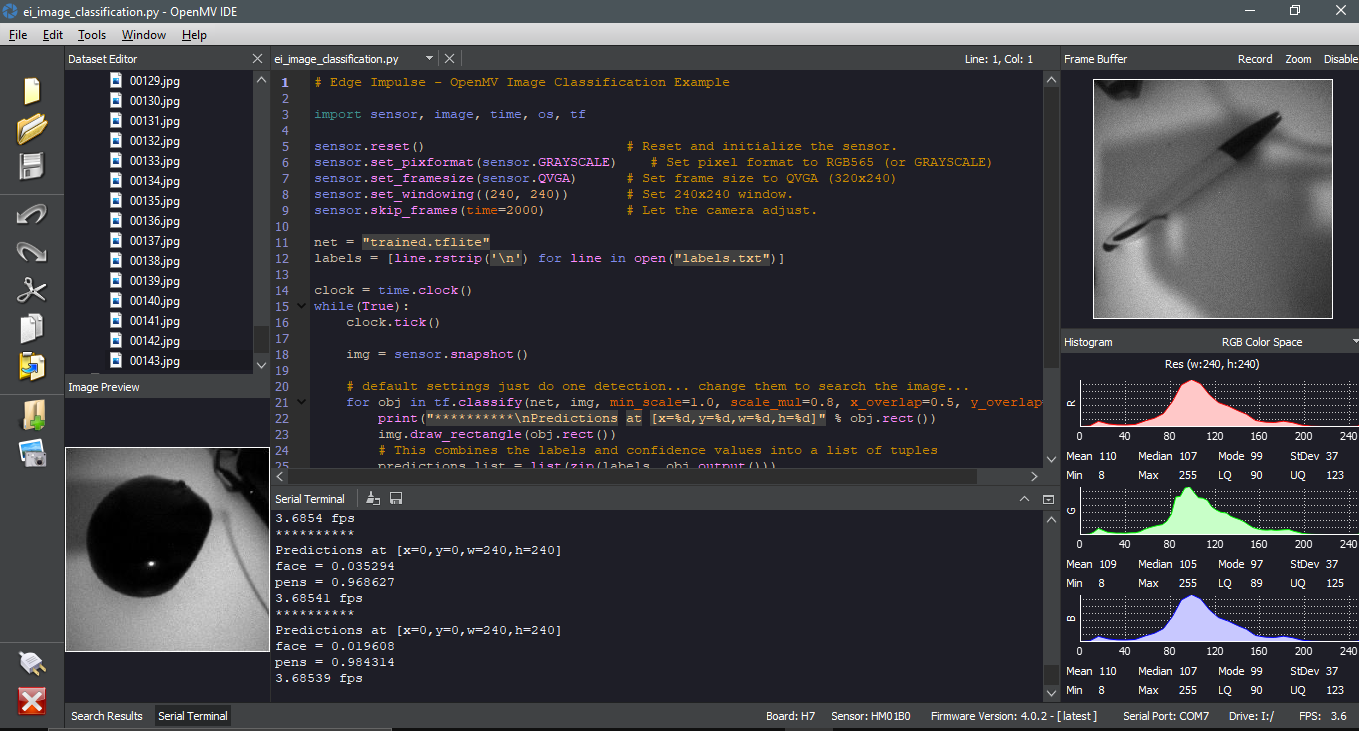
\includegraphics[width=\textwidth]{Arduino/Penoutput}
	\caption{Pen detection }
	\label{figure 9.13}
\end{figure}

\section{Face Detection using Edge Impulse}
In this model we will be detecting faces in an image without using the OpenMV IDE. We will be making use of Edge Impulse platform for training and testing the model.
The flowchart for the overall process is shown in the below figure \ref{figure 9.14} 
\begin{figure}[H]
	\centering
	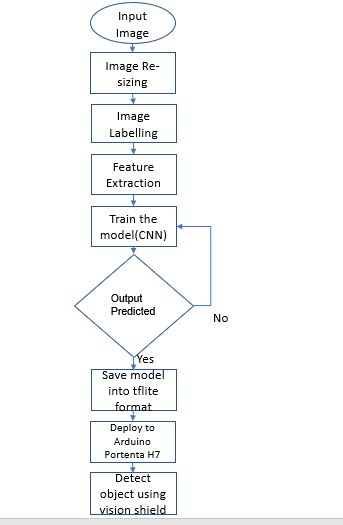
\includegraphics[width=\textwidth]{Arduino/flowchart2}
	\caption{Flowchart of the overall process }
	\label{figure 9.14}
\end{figure}

\subsection{Database}  To train a machine learning model for face detection we first need to find a database of images consisting of faces.  We can  create it by capturing the images using the Vision Shield camera. We can also download a dataset online and use it to train the model.  UTKFace  is one dataset with long age span(0 to 116 years old) consisting of over 20k single face images. We can download this dataset from the link \url{https://susanqq.github.io/UTKFace/}

\textbf{Selection of Dataset} : Manually captured images from the camera present on the Vision shield, Images taken from UTKFace dataset.
Training set : Consisting of 388 images
testing set : consisting of 98 images
In the below figure \ref{figure 9.115} we can see the sample images from UTKFace dataset. The dimension of the images in this dataset is 200x200 pixels. 
\begin{figure}[H]
	\centering
	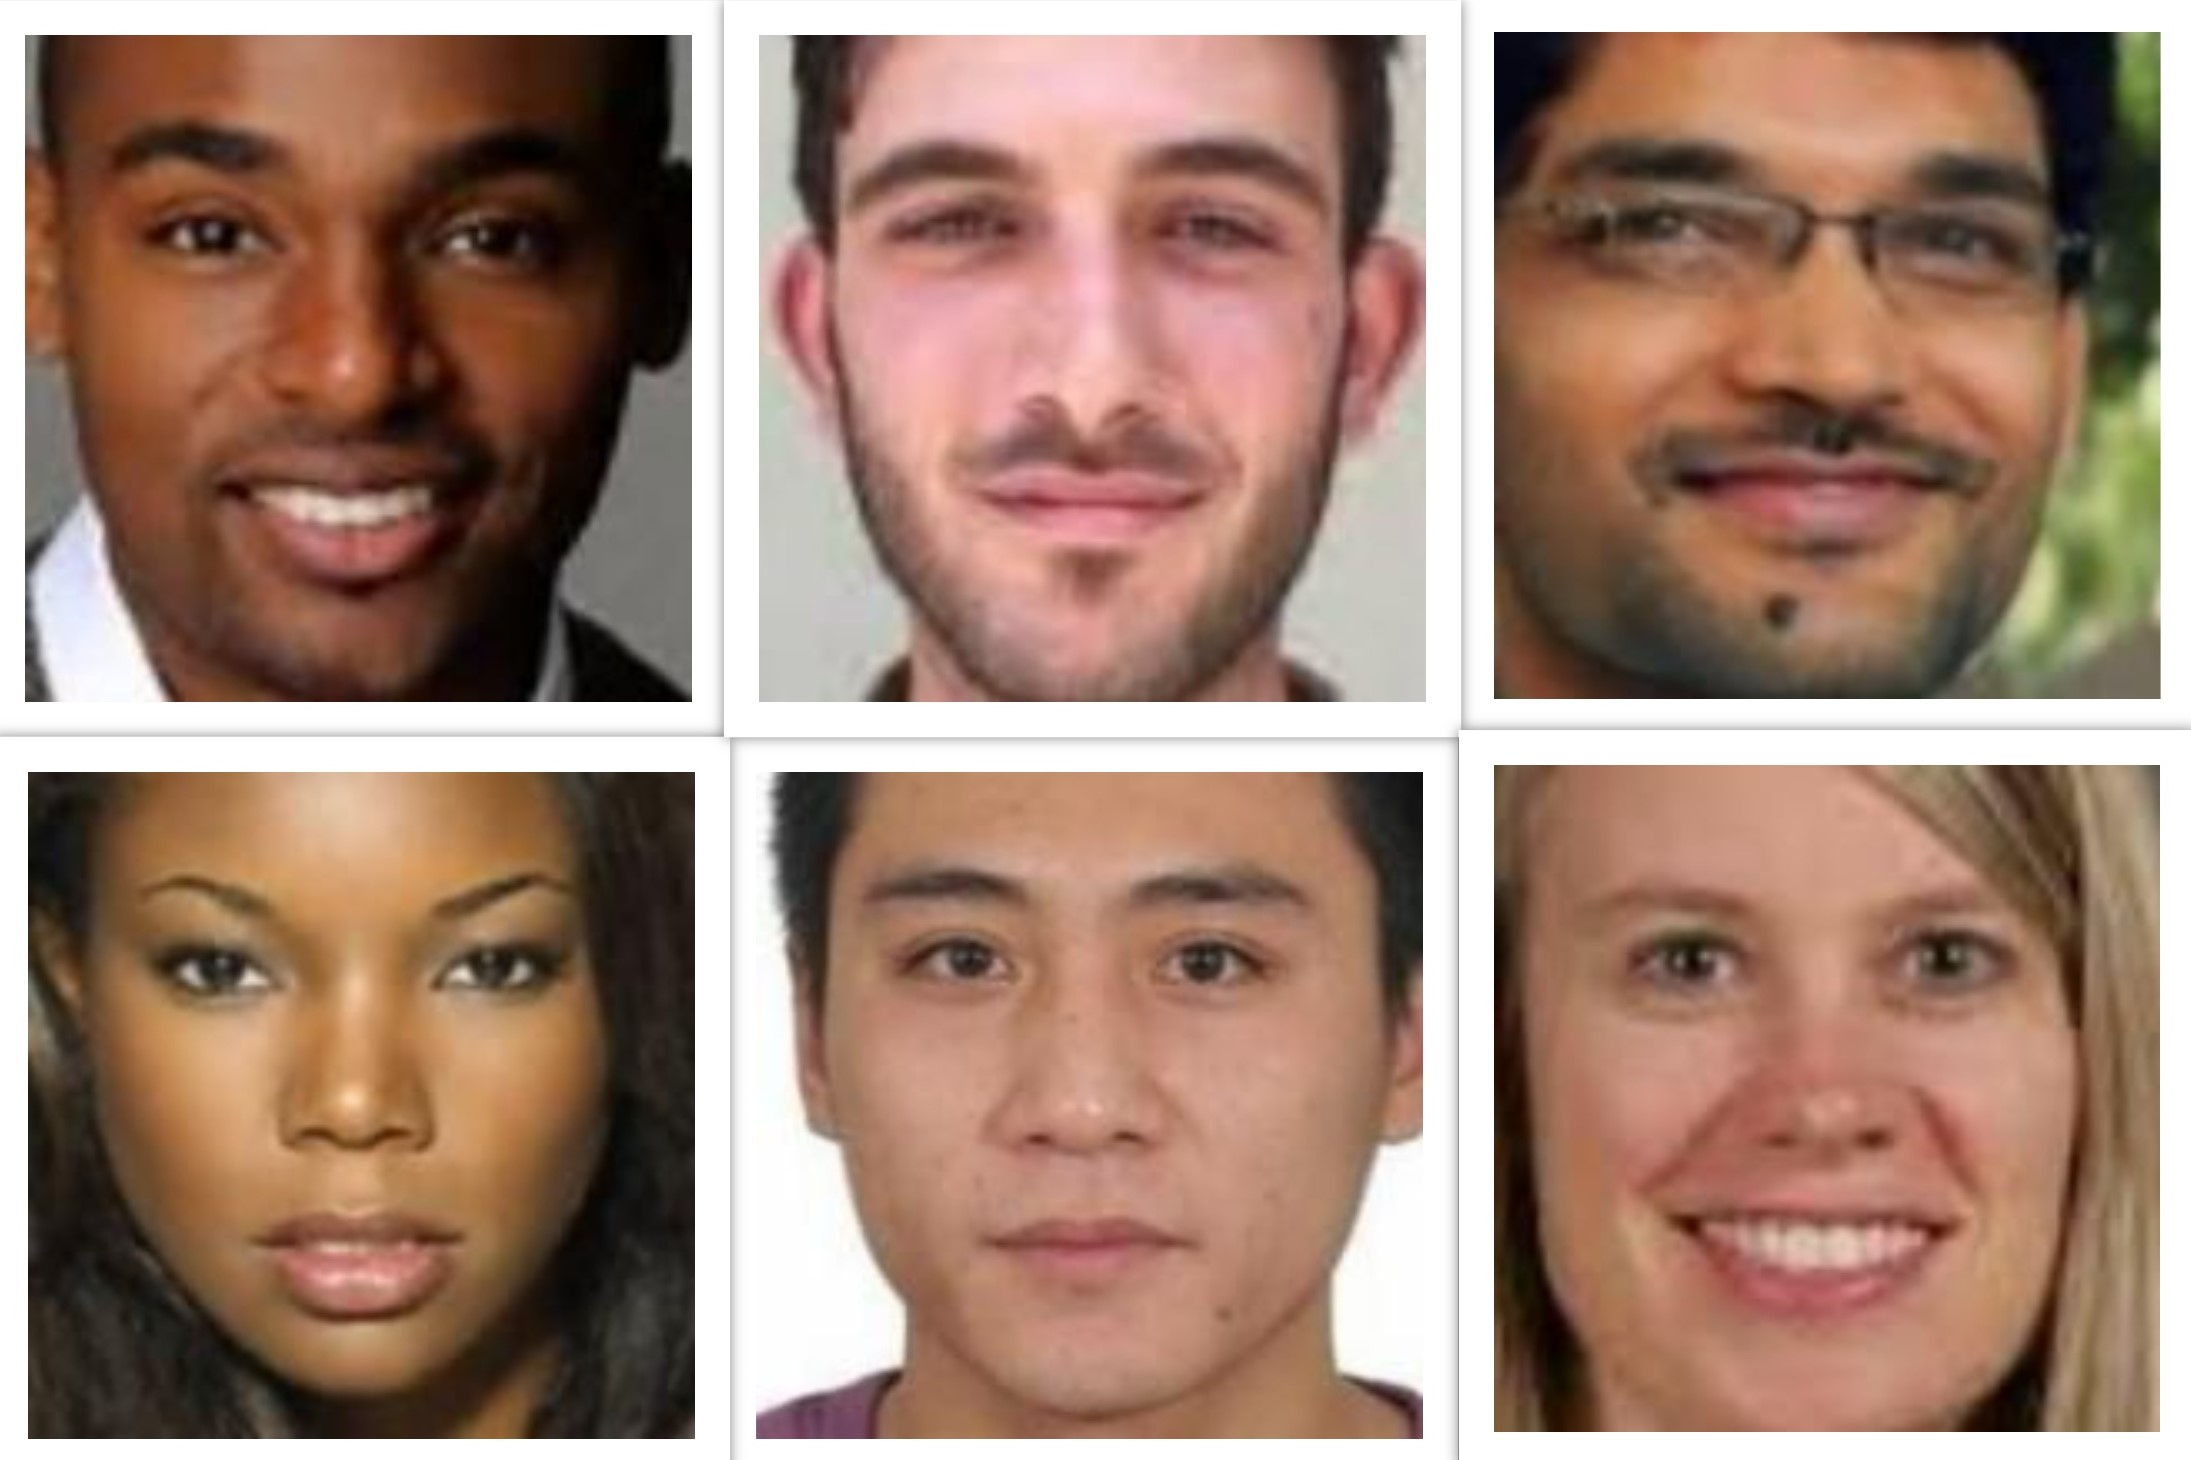
\includegraphics[width=\textwidth]{Arduino/sampldata}
	\caption{Sample Images from UTKFace Dataset  }
	\label{figure 9.115}
\end{figure}



\textbf{Uploading the dataset in the Edge Impulse} :
Firstly, we need to login in the Edge Impulse portal and create a project named Face\_detection. In order to upload our image dataset , we need to go to the Edge Impulse dashboard and click on acquire data and select  upload data. For uploading the dataset of images captured by Arduino Vision Shield, we need to connect it to the Edge Impulse Platform. This is described in the next section.


\subsection{Connecting the Arduino Portenta H7 with Edge Impulse}
In order to take pictures from the vision shield, we need to connect our device to the Edge Impulse portal and then start taking pictures. To do this,  we need to install the following software.

\begin{itemize}
	\item \textbf{Arduino CLI} : We need to download the Arduino CLI from the website \url{https://arduino.github.io/arduino-cli/latest/installation/} and extract the downloaded Zip file which is arduino-cli\_0.18.3\_Windows\_64bit and copy the path of the file which is \path{C:\Users\Shoeb\Downloads\arduino-cli_0.18.3_Windows_64bit.zip\}. Then we need to add this path in the Environment Variables list on our computer. After adding the path, we need to open command prompt and type Arduino-cli and press enter to install it. After the installation is done, type arduino-cli board list in the command prompt. It displays the device connected as Arduino Portenta H7 with port number and type as shown in the figure \ref{figure 9.16}.
		\begin{figure}[H]
			\centering
			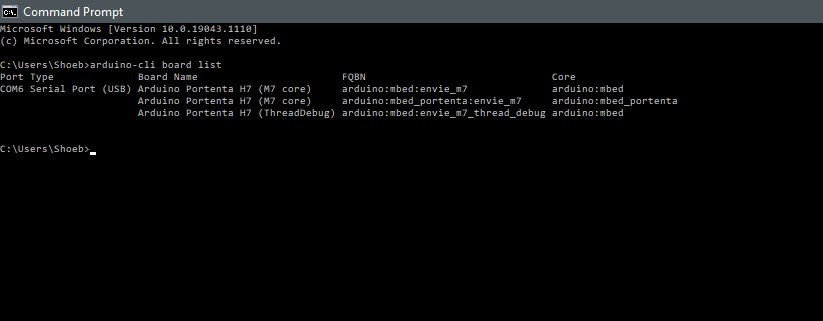
\includegraphics[width=\textwidth]{Arduino/arduino-cli}
			\caption{Arduino-CLI Installation }
			\label{figure 9.16}
		\end{figure}
		
		\item \textbf{Edge Impulse CLI } : We first need to install Python 3 and download Node.js version 14.17 or higher from the website \url{https://nodejs.org/en/}. The downloaded Windows installer file is named as node-v14.17.4-x64.msi. Then we need to begin installing by opening this Windows installer file. Click on install as shown in the figure.. and the installed path is \path{C:\ProgramData\Microsoft\Windows\Start Menu\Programs\Node.js} After the installation is done   we need to open the command prompt and type npm install -g edge-impulse-cli --force to install it.
		
		\begin{figure}[H]
			\centering
			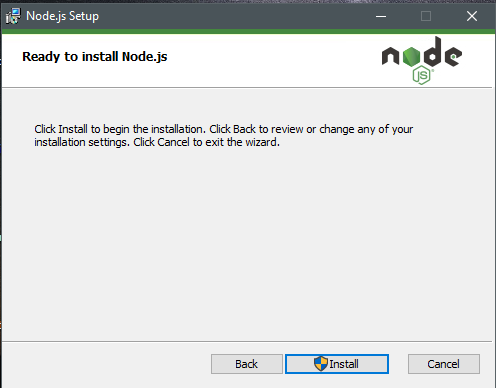
\includegraphics[width=\textwidth]{Arduino/nodejs}
			\caption{Node.js Installation }
			\label{figure 9.17}
		\end{figure}
		
		
	\end{itemize}
	
	
	After installing these two softwares, we need to connect the Arduino Portenta H7 with Edge Impulse. To do this, we need to download the latest Edge Impulse firmware from the website \url{https://docs.edgeimpulse.com/docs/arduino-portenta-h7}. The downloaded file is named as arduino-portenta-h7-preview.zip . We ned to extract this file and open the flash script for Windows which is present inside the folder named as flash\_windows.bat. After the flashing is done, we need to press the reset button once to launch the new firmware. Now we need to open the command prompt and type edge-impulse-daemon. This prompts us to login with our Edge Impulse ID and Password in the command prompt. After the login is succesful,we need to name the device, here i have named it as Arduino Portenta H7 as shown in the figure \ref{figure 9.18}.
	
	\begin{figure}[H]
		\centering
		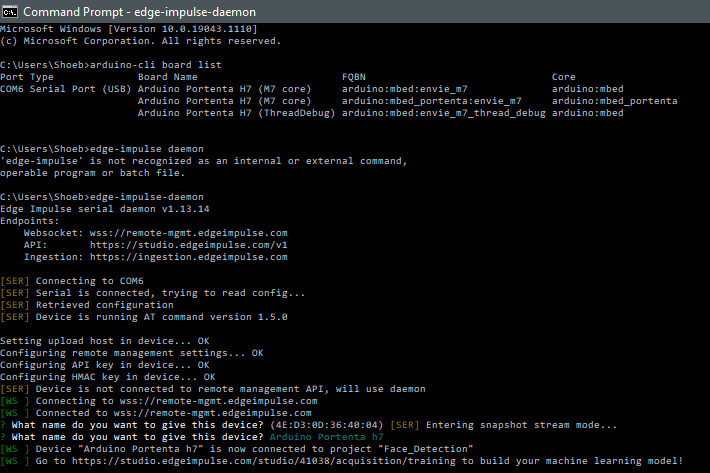
\includegraphics[width=\textwidth]{Arduino/edgecli}
		\caption{Connecting Arduino Portenta H7 with Edge Impulse }
		\label{figure 9.18}
	\end{figure}
	
	
	
	To verify that the board is connected, go to the Edge Impulse website and click on devices,we can see that our device is connected as shown in the figure \ref{figure 9.19}. This way we have successfully connected our board with the Edge Impulse platform and now we can go for training the model.
	\begin{figure}[H]
		\centering
		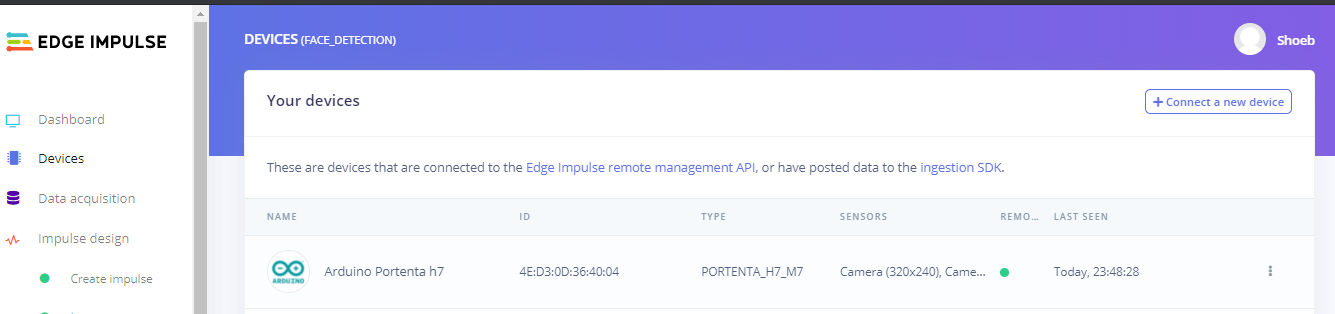
\includegraphics[width=\textwidth]{Arduino/connectededge}
		\caption{Connected  Devices in the Edge Impulse}
		\label{figure 9.19}
	\end{figure}
	\subsection{Data Labelling}
	Now that our data is uploaded, we need to label the data. To do this, we go to Labeling queue option in Data Acquisition and start drawing bounding box around the object and label it. In our database we have two different objects which are faces and pens. So we manually draw bounding box around the object and label them for all the images in the dataset.
	\begin{figure}[H]
		\centering
		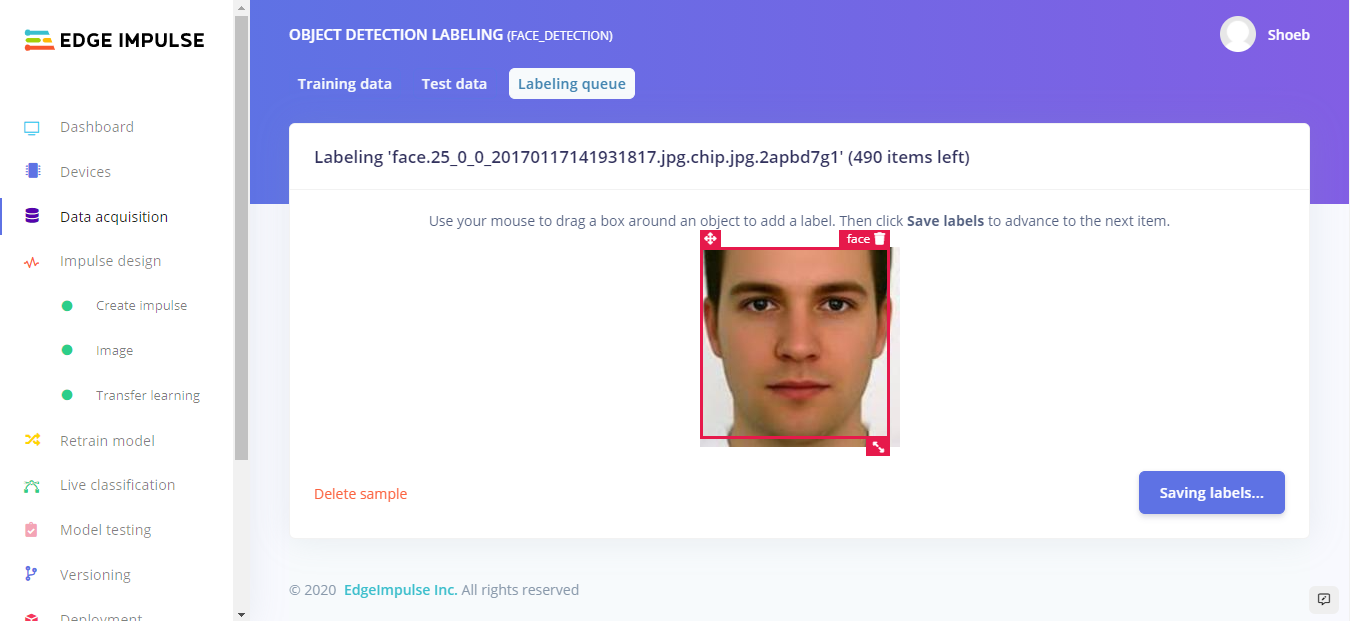
\includegraphics[width=\textwidth]{Arduino/labelface}
		\caption{Labelling an Image }
		\label{figure 9.15}
	\end{figure}
	\section{Data transformation} 
	\subsection{Designing the Impulse}
	\textbf{Image Preprocessing} :
	
	For designing the impulse, click on Impulse design and then set the image width and height to 320X320 because the object detection pre-trained model works only with images of size 320X320 \cite{EdgeImpulse:2021}.Then in the processing block we click on Image. The image pre-processing block takes input image and can optionally convert it into grayscale and then turns the data into a features array.  We then click on learning block and select object detection. Then click on save impulse as hown in the figure \ref{figure 9.20}.
	\begin{figure}[H]
		\centering
		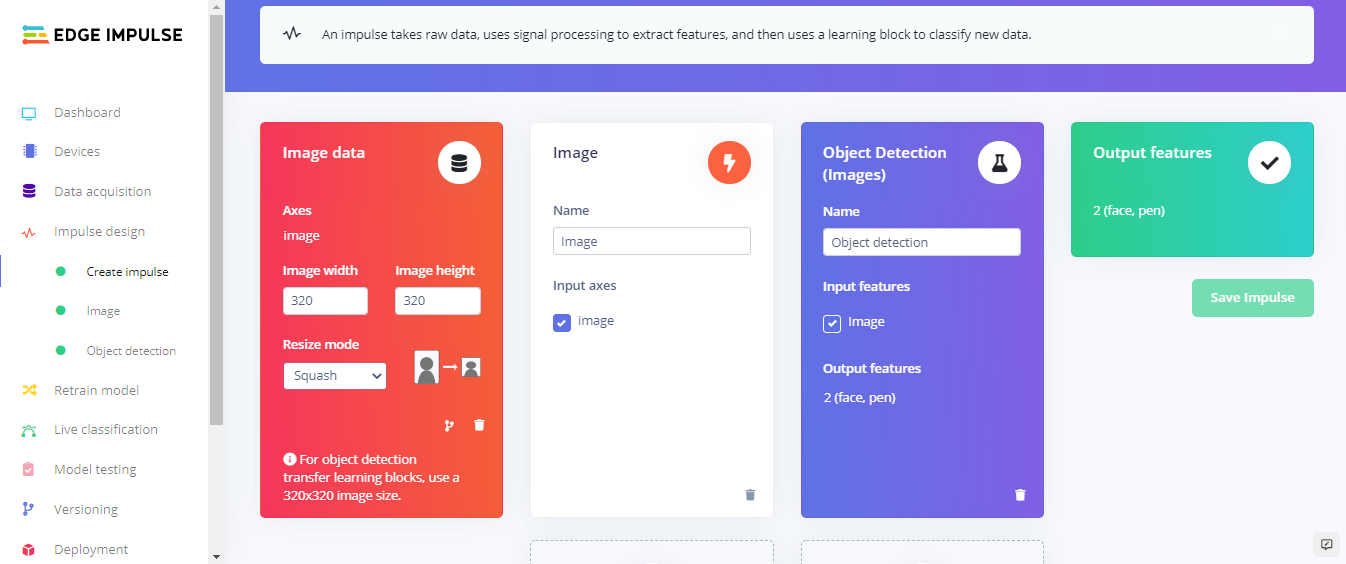
\includegraphics[width=\textwidth]{Arduino/createimpulse}
		\caption{Create Impulse}
		\label{figure 9.20}
	\end{figure}
	\subsection{Configuring the Image processing block } 
	To configure the processing block, click Images in the menu on the left. This will show us  the raw data on top of the screen and the results of the processing step on the right. we can also use the options to switch between 'RGB' and 'Grayscale' mode. We then click on save parameters as shown in figure \ref{figure 9.21}. 
	\begin{figure}[H]
		\centering
		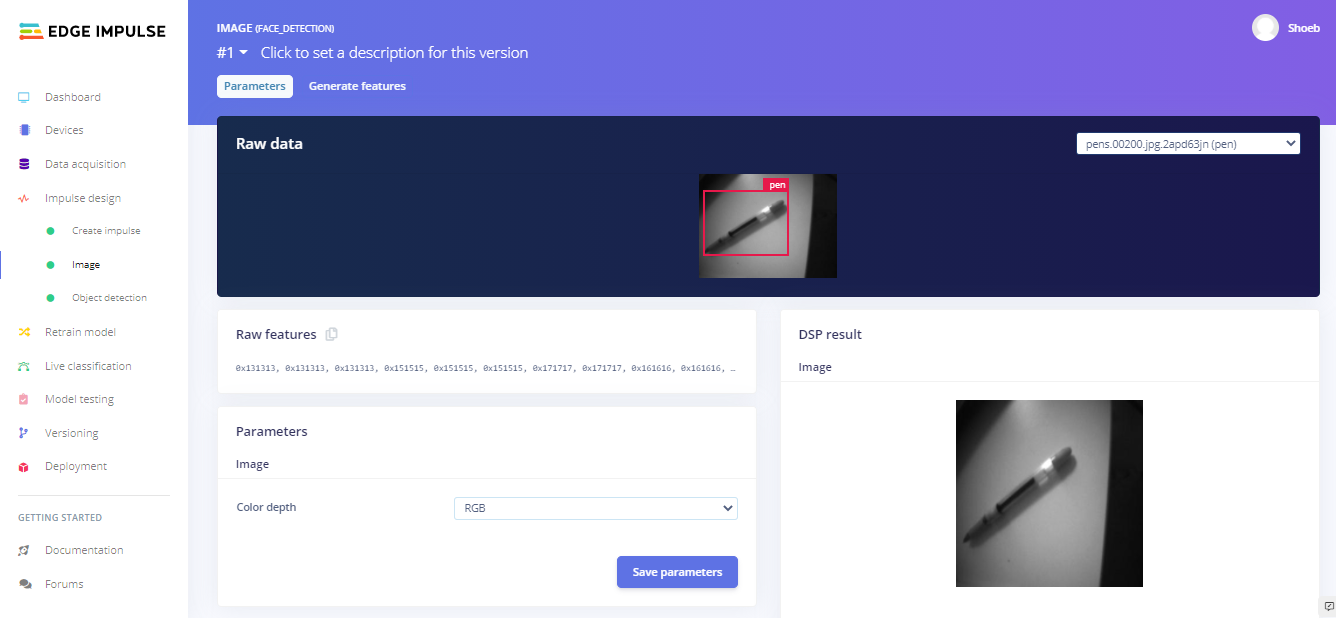
\includegraphics[width=\textwidth]{Arduino/saveparameters}
		\caption{Save parameters}
		\label{figure 9.21}
	\end{figure}
	
	Then click on generate features option on the top and then click on generate features. In the figure \ref{figure 9.22} we can see that features generated from the dataset of images consisting of pens and faces are easily distinguishable.
	\begin{figure}[H]
		\centering
		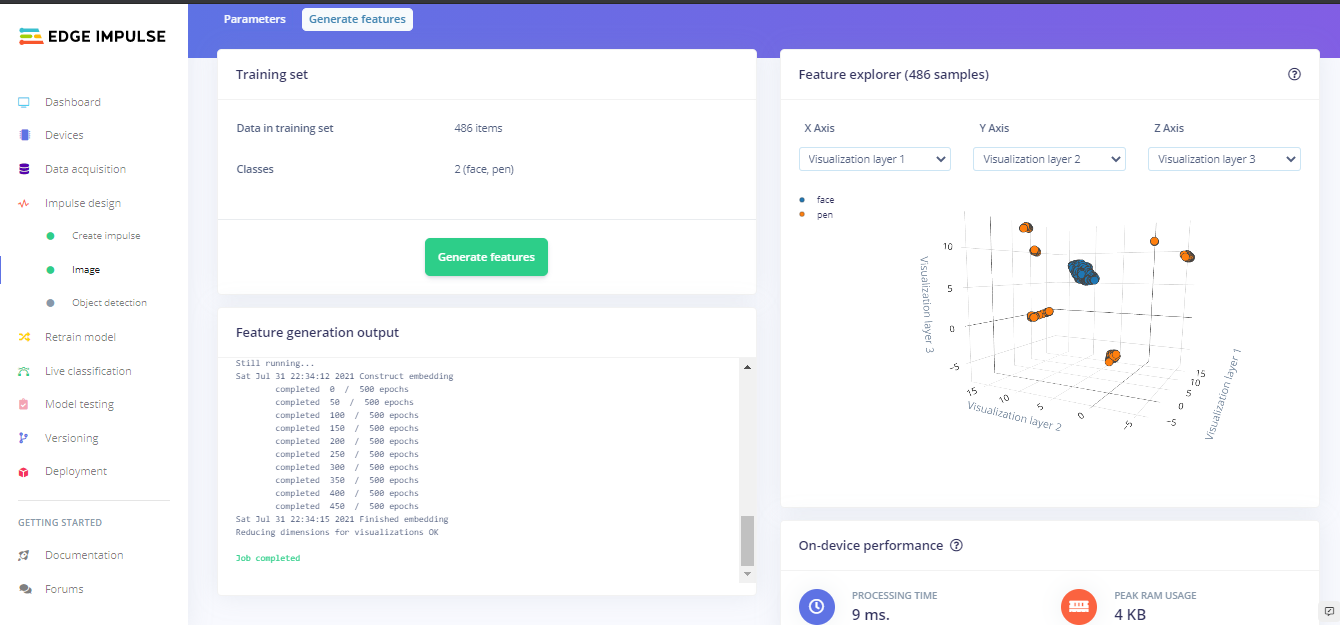
\includegraphics[width=\textwidth]{Arduino/featuregenerate}
		\caption{Generate Features}
		\label{figure 9.22}
	\end{figure}
	\section{Data training}
	\textbf{Configuring the transfer learning model} :
	
	Here we are using transfer learning block because it is easier to use a pre-trained model by only retaining the upper layers of a neural network and then we can train the model in a short time. To configure the transfer learning model, click on object detection. Here, we can set the learning rate ,in our case we have set it to 0.15 and  the number of training cycles to 25. Then we select the base model, here we have selected as MobileNetV2 and then click on start training.  After the training process is completed we can see from the figure \ref{figure 9.23} the precision of it is 87\%.
	\begin{figure}[H]
		\centering
		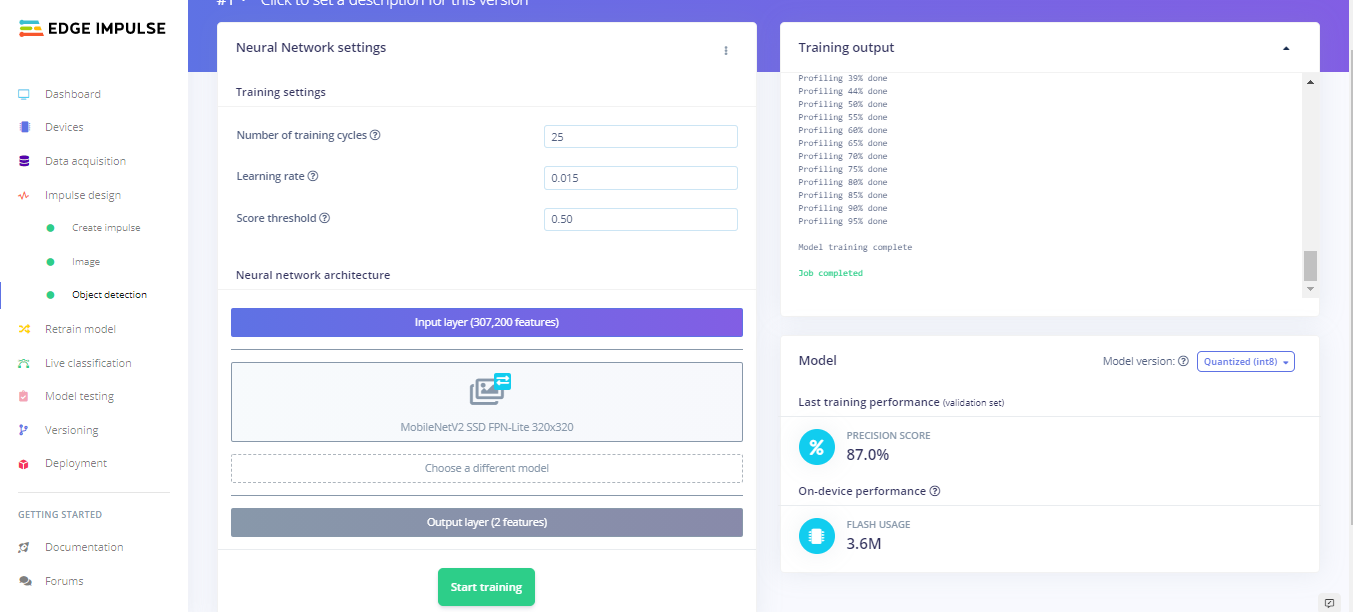
\includegraphics[width=\textwidth]{Arduino/Trainedmodel}
		\caption{Completed training}
		\label{figure 9.23}
	\end{figure}
	\section{Testing the model }
	In order to test the model, we need to click on the option model testing and then click on classify all. Here, the dataset images were automatically divided into training and testing images. Here, the model divided the input images into training images consisting of 388 images and testing consisting of 98 images. The testing images are then used to check how well the model performs. As we can see from the figure \ref{figure 9.24} that the model achieved 87.1\% accuracy.
	
	\begin{figure}[H]
		\centering
		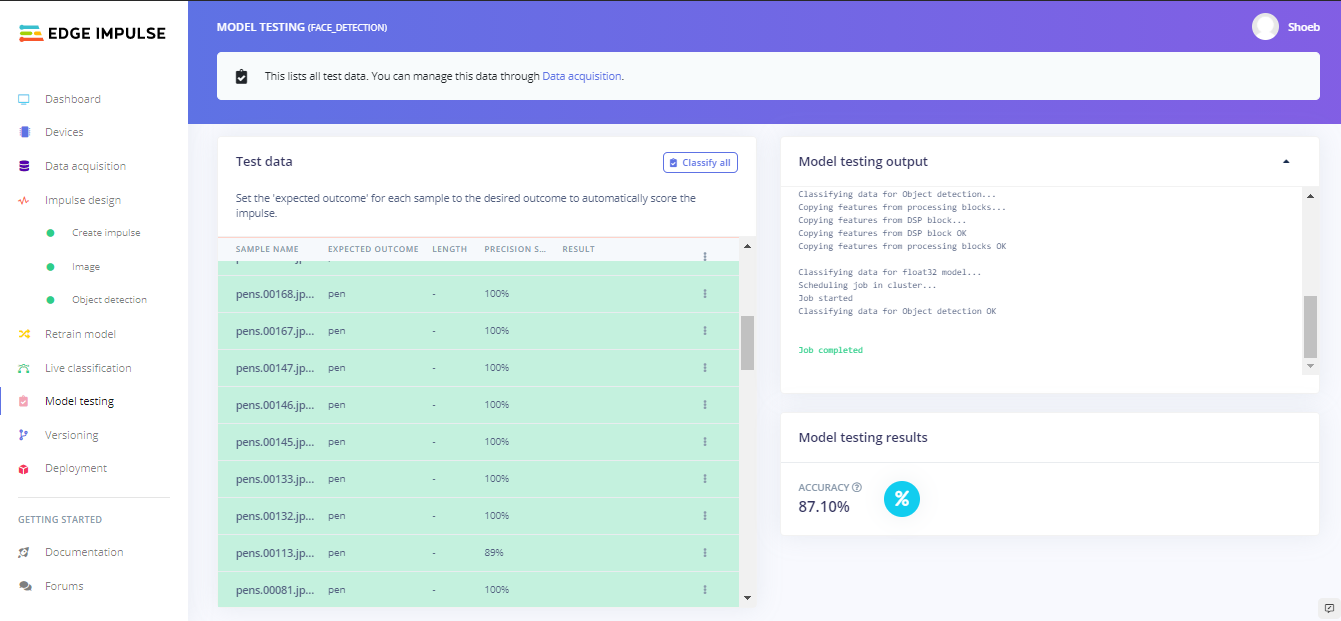
\includegraphics[width=\textwidth]{Arduino/testmodel}
		\caption{Testing the model}
		\label{figure 9.24}
	\end{figure}
	
	We can also do the live classification and detect objects in real time using the vision shield.  Click on the live classification option in the menu and connect our Portenta H7 device with the Edge Impulse by selecting the device. Then as soon as it is connected we can see the camera stream from vision shield. Here we have tested the model by focusing on face and as we can se from the figure \ref{figure 9.25} that it gives the output as face with 0.89 value which is a pretty good prediction.
	\begin{figure}[H]
		\centering
		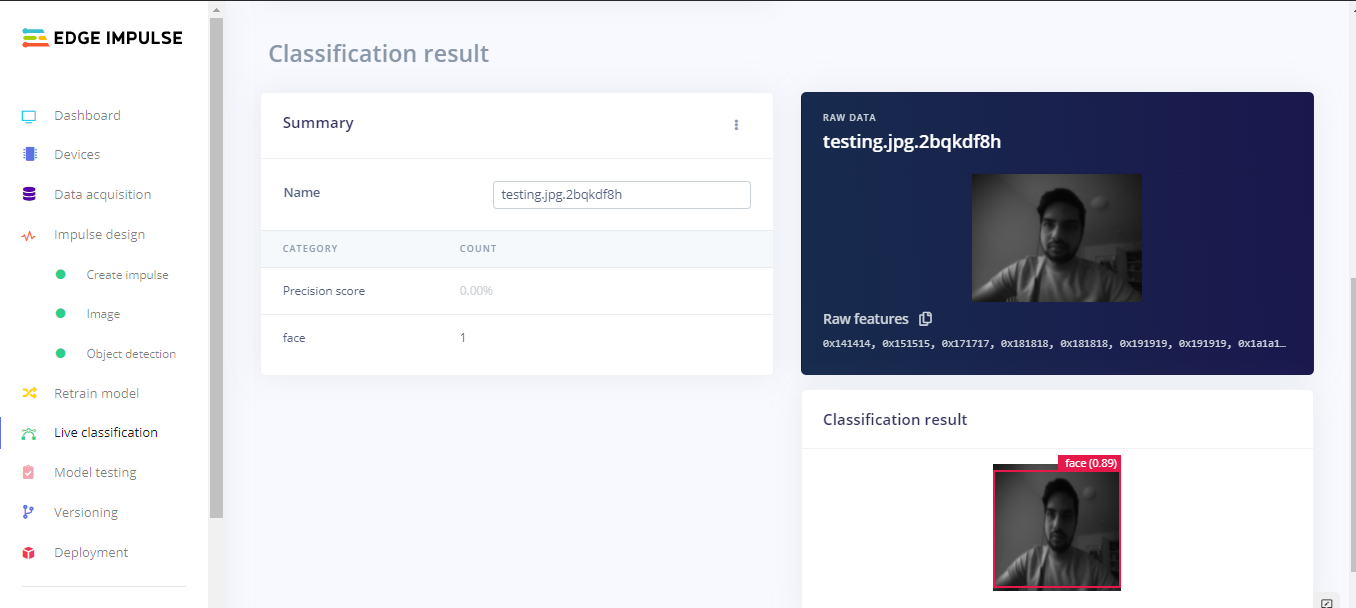
\includegraphics[width=\textwidth]{Arduino/liveclassification}
		\caption{Live classification by using vision shield camera}
		\label{figure 9.25}
	\end{figure}
	
	
	\chapter{Use TensorFlow Lite with Portenta H7}
	
	\section{Introduction}
	In this chapter, we will be using Google Colab to train an object detection model and then convert it to TensorFlow Lite format in order to upload and validate  it on Arduino Portenta H7. TensoFlow Lite for microcontrollers is designed to run machine learning models with limited memory. TensorFlow Lite for microcontrollers is written in C++ 11 and needs a 32-bit platform.  Arduino Portenta H7 board is not yet supported to run TensorFlow Lite models using Arduino IDE \cite{GoogleTensorFlowLite:2021}, but it is worth giving a try.
	\section{Training a Face detection model using Google Colaboratory}
	\subsection{Google Colaboratory}
	Google Colaboratory or Colab is a product from Google Research and  is a free Jupyter notebook environment running completely in the cloud. It is typically well suited to machine learning and data analysis. The good thing is it requires no set up and provides free access to computing resources like GPU and TPU \cite{GoogleColab:2021}.
	
	
	\textbf{Advantages of Colab} 
	\begin{itemize}  
		\item \textbf{Pre installed libraries}: It provides pre-installed machine learning libraries including PyTorch, Keras, TensorFlow
		\item \textbf{Saved on the Cloud} : If we use a Jupyter notebook, then everything is saved on a local device. However, when we use Google Colab, we can sasve it on the cloud and can access from any device by just signing in Google Drive account.
		\item \textbf{Collaboration} : It helps in providing access to multiple developers working on the project to edit the code or code together and also share the completed code with the developers
		\item \textbf{Free GPU and TPU use} : 
		This is probably the best feature as Google Research lets us use their dedicated GPUs and TPUs for our personal machine learning projects. Therefore, our computers don?t have to undergo the complex computations while training the model because it is done on the cloud
		
	\end{itemize}
	
	\section{Database}
	The Database for faces is the same as in the previous chapter which is UTKFace Dataset. We will be training the model based on Image classification technique so we will be using another class that is Flowers in our case and the database for it can be downloaded from Google.
	\textbf{Selection of Dataset} : Images taken from Flowers dataset :100 images consisting of Roses saved in a folder named as Roses. The dimensions of the images in the dataset varies but we select images of dimensions in the range of 224 x 224 pixels. 
	\begin{figure}[H]
		\centering
		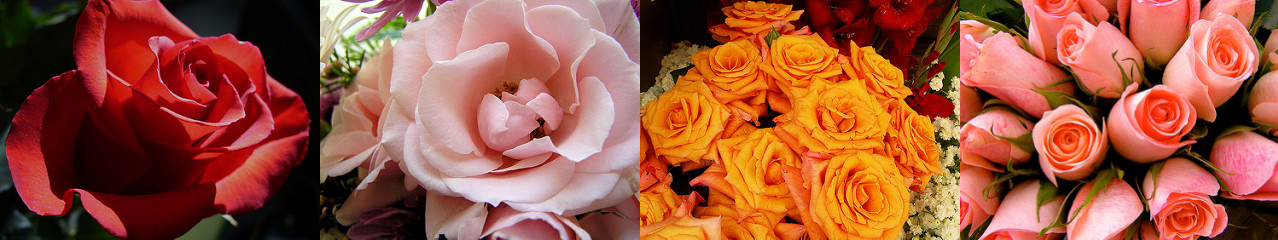
\includegraphics[width=\textwidth]{Arduino/roses}
		\caption{Sample Images from flowers dataset}
		\label{figure 10.1}
	\end{figure}
	Images taken from UTKFace dataset : 120 images consisting of Faces in a folder saved as Faces. The dimensions of the images is 200X200 pixels.
	\subsection{Connecting to Google Drive}
	In order to create and save notebook in Colab, we need to connect it to our Google Drive. Also, we need to upload our images dataset in our Google Drive in order to access it from Colab. To do this,we use the function \PYTHON{drive.mount('/content/gdrive')}. This will redirect to our google sign-in page and gives us the authorization key required to connect our Google Drive to Colab. After entering the key we will be connected to our Google Drive.
	
	
	
	\subsection{Setting up the Dataset}
	This section  is a significant part of where we have placed our image zipped file and this .ipynb script file(base\_path) on our Google Drive, how we have named our zipped file(imagezipped) which in our case is 'images\_RF.zip'. and the name of the folder(data\_dir) which is data\_dir='images'where we compiled our images before compressing it.
	\begin{figure}[H]
		\centering
		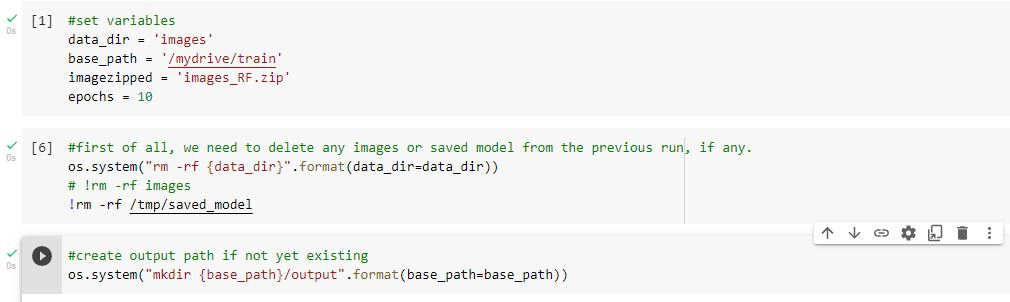
\includegraphics[width=\textwidth]{Arduino/setdataset}
		\caption{Setting up the dataset}
		\label{figure 10.2}
	\end{figure}
	\section{Data Preprocessing}
	\textbf{Rescaling} :
	
	In the preprocessing part we will be first rescaling the image using the rescaling function \PYTHON{rescale=1./255} because our original images consist in RGB coefficients in the 0-255, but such values would be too high for our model to process (given a typical learning rate), so we target values between 0 and 1 instead by scaling with a 1/255 factor. 
	
	\textbf{Data Augmentation} :
	
	In the data augmentation part, we will be using image augmentation techniques such as  rotation of images and horizontal flipping of images.  Here, the rotation range of images is given as 40 degrees as shown in figure \ref{figure 10.3}.
	\begin{figure}[H]
		\centering
		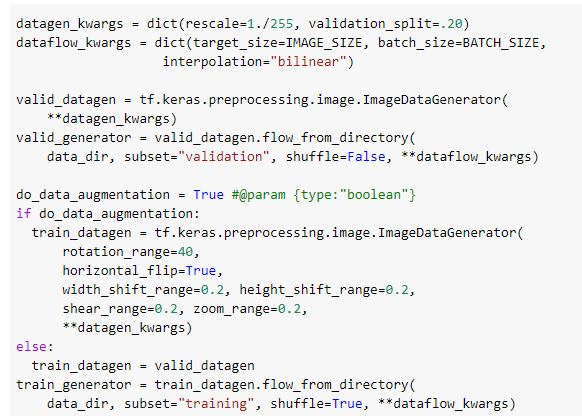
\includegraphics[width=\textwidth]{Arduino/rescaling}
		\caption{Rescaling and Data Augmentation}
		\label{figure 10.3}
	\end{figure}
	
	\section{Training the model}
	In this we have used a pre-trained image classification model based on MobileNet V2(224x224). The input image size should be in 224x224 pixels dimension. The model here is build with keras sequential layers and the drop out rate given here is 0.2. The batch-size is 32 and the optimizer used in this model is Stochastic gradient descent(SGD) with a learning rate of 0.005. The loss function used here is Categorical cross entropy. we have set the epoch value to 10.Epoch is the number of iteration for back propagation to correct the errors on earlier part so that it would increase accuracy. The larger the epoch the more iteration thus the longer the training process.
	
	\begin{figure}[H]
		\centering
		\includegraphics[width=\textwidth]{Arduino/trainingmodel}
		\caption{Training the model}
		\label{figure 10.4}
	\end{figure}
	
	\section{Testing the model}
	Here, we will be testing the model on an image from validation dataset. As can be seen from the figure  \ref{figure 10.5} , the model predicts the output which is face in the image accurately.
	\begin{figure}[H]
		\centering
		\includegraphics[width=\textwidth]{Arduino/testing}
		\caption{Testing the model}
		\label{figure 10.5}
	\end{figure}
	The trained model can then be stored on session storage.
	
	\section{Converting the saved model to tflite format}

To convert the saved model in to tflite format we use the following function \PYTHON{converter = tf.lite.TFLiteConverter.from\_saved\_model(saved\_model)}

After converting the model into tflite we save the tflite file on our drive. The next step is to convert the tflite file to C++ format so that we can upload the program in the Arduino IDE.

\section{Converting the tflite file to Arduino header file}
	In order to run the object detection model in Arduino IDE we need to program our model in C++ format and also add the arduino header file created from our tflite model. To create a arduino header file, we use Gitpod to convert tflite file to a header(.h file) file. TO do this, firstly we need to login to GitPod using our GitHub credentials. Then we need to create a new workspace. In the command terminal we need to use this command \PYTHON{xxd -i model.tfite model.h}.
	This will generate a header file we need in our C++ program to upload in the Arduino IDE. After downloading the header file, we need to copy the contents of the file and paste it in our program with the command \PYTHON{const unsigned char model\_tflite[] = }. This represents the features of our face detection model. Then we need to implement the face detection function in C++ code.
	\section{Open Questions}
	\subsection{Arduino Portenta H7 board not compatible for object detection using Arduino IDE}
	The problem occured duing the implementation of face detection model using Arduino IDE is that there is no previous work done on object detection using Arduino Portenta H7 board as it was not comptabile\cite{GoogleTensorFlowLite:2021}.Therefore, there was no data avalaible which could be taken as a reference for our face detection model. Also to implement a TensorFlowLite model in the Arduino IDE is a herculian task as our board is not fast enough and the  time to compile a program is more than 20 minutes and there are no libraries available to implement the object detection model. However, there is only one example available online which is the Hello World example of Arduino also called as a sine wave function in a tflite format which can be executed using the Arduino IDE but we cannot take this as a reference because object detection model and a sine wave model are completely different. 
	\subsubsection{Possible Solution}
	The possible solution could be using OpenMV IDE instead of Arduino IDE. OpenMV IDE has more number of functions when compared to Arduino IDE such as uploading dataset real-time by capturing images from vision shield. It also has many more example programs like face tracking, face filter. So, using OpenMV IDE could be a better and easy solution for this issue. 
	\subsection{Unable to Deploy object detection model trained on Edge Impulse using Arduino IDE }
	The object detection model which was trained for face detection in edge impulse platform and the tflite file generated online was unable to deploy on Arduino IDE. The model works completely fine on the platform, however during deployment on Arduino Portenta H7 board using Arduino IDE received various errors. Upon consulting the edge impulse platform creators we got to know that they are not yet ready in deployment of the model generated from their platform  using arduino IDE.
	\subsubsection{Possible Solution}
	The model generated from Edge Impulse platform is coded in python programming language. For Arduino IDE, the programming language is C++. So, as of now Edge Impulse does have some issues when it comes to Arduino IDE as some changes has to be done. So, the better soultion would be using OpenMV IDE, as it supports MicroPython and the Edge Impulse model generates a python file which we can upload in OpenMV IDE and implement our face detection model.
	
	\chapter{Source Code}
	
	\section{Serial Blink Example for Arduino Portenta H7 }

	\begin{verbatim}
		
		void setup() {
			Serial.begin(115200);    // Sets the data rate in bits per second (baud) for serial data transmission
			pinMode(LEDR, OUTPUT);   // LEDB = blue, LEDG or LED_BUILTIN = green, LEDR = red (typically for errors)
			#ifdef CORE_CM7          // shows how to specifiy a specific core 
			bootM4();
			#endif
		}
		
		void loop() {
			Serial.println("Serial print works on the M7 core, just ignored on the M4 Core, unless you use RPC!");
			digitalWrite(LEDR, LOW);   // Portenta onboard LED connected to 3V3 so ground it to light
			delay(1000);               // wait for a second
			digitalWrite(LEDR, HIGH);  // turn the LED off by not grounding it, weird eh.
			delay(4000);               // wait for 3 seconds
		}
	\end{verbatim}

	\section{Example Script for blinking builtin RGB LED on the Arduino Portenta H7 with OpenMV}

	\begin{verbatim}
		import pyb
		redLED = pyb.LED(1) # built-in red LED
		greenLED = pyb.LED(2) # built-in green LED
		blueLED = pyb.LED(3) # built-in blue LED
		while True:
		# Turns on the red LED
		redLED.on()
		# Makes the script wait for 1 second (1000 miliseconds)
		pyb.delay(1000)
		# Turns off the red LED
		redLED.off()
		pyb.delay(1000)
		greenLED.on()
		pyb.delay(1000)
		greenLED.off()
		pyb.delay(1000)
		blueLED.on()
		pyb.delay(1000)
		blueLED.off()
		pyb.delay(1000)
	\end{verbatim}


	\section{QR Code Information Extraction Program}

	\begin{verbatim}
		import sensor, image, time
		
		sensor.reset()
		sensor.set_pixformat(sensor.RGB565)
		sensor.set_framesize(sensor.QVGA)
		sensor.skip_frames(time = 2000)
		sensor.set_auto_gain(False) # must turn this off to prevent image washout...
		clock = time.clock()
		
		while(True):
		clock.tick()
		img = sensor.snapshot()
		img.lens_corr(1.8) # strength of 1.8 is good for the 2.8mm lens.
		for code in img.find_qrcodes():
		img.draw_rectangle(code.rect(), color = (255, 0, 0))
		print(code)
		print(clock.fps())
		
	\end{verbatim}

	\section{Finding Circles around the Objects}

	\begin{verbatim}
		import sensor, image, time
		
		sensor.reset()
		sensor.set_pixformat(sensor.GRAYSCALE) # grayscale is faster
		sensor.set_framesize(sensor.QQVGA)
		sensor.skip_frames(time = 2000)
		clock = time.clock()
		
		while(True):
		clock.tick()
		img = sensor.snapshot().lens_corr(1.8)
		
		# Circle objects have four values: x, y, r (radius), and magnitude. The
		# magnitude is the strength of the detection of the circle. Higher is
		# better...
		
		# `threshold` controls how many circles are found. Increase its value
		# to decrease the number of circles detected...
		
		# `x_margin`, `y_margin`, and `r_margin` control the merging of similar
		# circles in the x, y, and r (radius) directions.
		
		# r_min, r_max, and r_step control what radiuses of circles are tested.
		# Shrinking the number of tested circle radiuses yields a big performance boost.
		
		for c in img.find_circles(threshold = 2000, x_margin = 10, y_margin = 10, r_margin = 10,
		r_min = 2, r_max = 100, r_step = 2):
		img.draw_circle(c.x(), c.y(), c.r(), color = (255, 0, 0))
		print(c)
		
		print("FPS %f" % clock.fps())
		
	\end{verbatim}

	\section{Creating a basic face filter with OpenMV}

	\begin{verbatim}
		import sensor # Import the module for sensor related functions
		import image # Import module containing machine vision algorithms
		import time # Import module for tracking elapsed time
		
		sensor.reset() # Resets the sensor
		sensor.set_contrast(3) # Sets the contrast to the highest level (min -3, max 3)
		sensor.set_gainceiling(16) # Sets the amplification of camera sensor signal
		
		# HQVGA and GRAYSCALE are the best for face tracking.
		sensor.set_framesize(sensor.HQVGA)
		sensor.set_pixformat(sensor.GRAYSCALE)
		
		# Load the built-in frontal face Haar Cascade
		# By default this will use all stages, lower stages is faster but less accurate.
		face_cascade = image.HaarCascade("frontalface", stages=25)
		print(face_cascade) # Prints the Haar Cascade configuration
		
		faceImage = image.Image("/face.pbm", copy_to_fb=False) # Loads a bitmap file from the flash storage
		clock = time.clock() # Instantiates a clock object to calculate the FPS
		
		while (True):
		clock.tick() # Advances the clock
		cameraImage = sensor.snapshot() # Takes a snapshot and saves it in memory
		
		# Find objects.
		# Note: Lower scale factor scales-down the image more and detects smaller objects.
		# Higher threshold results in a higher detection rate, with more false positives.
		boundingBoxes = cameraImage.find_features(face_cascade, threshold=1, scale_factor=1.5)
		
		# Draw objects
		for boundingBox in boundingBoxes:
		faceX = boundingBox[0]
		faceY = boundingBox[1]
		faceWidth = boundingBox[2]
		
		# Calculates the scale ratio to scale the bitmap image to match the bounding box
		scale_ratio = faceWidth / faceImage.width()
		# Draws the bitmap on top of the camera stream
		cameraImage.draw_image(faceImage, faceX, faceY, x_scale=scale_ratio, y_scale=scale_ratio)
		
		
		# Print FPS.
		# Note: The actual FPS is higher when not displaying a frame buffer preview in the IDE
		print(clock.fps())
		
	\end{verbatim}

	\section{Face Tracking}

	\begin{verbatim}
		import sensor, time, image
		
		# Reset sensor
		sensor.reset()
		sensor.set_contrast(3)
		sensor.set_gainceiling(16)
		sensor.set_framesize(sensor.QVGA)
		sensor.set_windowing((320, 240))
		sensor.set_pixformat(sensor.GRAYSCALE)
		
		# Skip a few frames to allow the sensor settle down
		sensor.skip_frames(time = 2000)
		
		# Load Haar Cascade
		# By default this will use all stages, lower satges is faster but less accurate.
		face_cascade = image.HaarCascade("frontalface", stages=25)
		print(face_cascade)
		
		# First set of keypoints
		kpts1 = None
		
		# Find a face!
		while (kpts1 == None):
		img = sensor.snapshot()
		img.draw_string(0, 0, "Looking for a face...")
		# Find faces
		objects = img.find_features(face_cascade, threshold=0.5, scale=1.25)
		if objects:
		# Expand the ROI by 31 pixels in every direction
		face = (objects[0][0]-31, objects[0][1]-31,objects[0][2]+31*2, objects[0][3]+31*2)
		# Extract keypoints using the detect face size as the ROI
		kpts1 = img.find_keypoints(threshold=10, scale_factor=1.1, max_keypoints=100, roi=face)
		# Draw a rectangle around the first face
		img.draw_rectangle(objects[0])
		
		# Draw keypoints
		print(kpts1)
		img.draw_keypoints(kpts1, size=24)
		img = sensor.snapshot()
		time.sleep_ms(2000)
		
		# FPS clock
		clock = time.clock()
		
		while (True):
		clock.tick()
		img = sensor.snapshot()
		# Extract keypoints from the whole frame
		kpts2 = img.find_keypoints(threshold=10, scale_factor=1.1, max_keypoints=100, normalized=True)
		
		if (kpts2):
		# Match the first set of keypoints with the second one
		c=image.match_descriptor(kpts1, kpts2, threshold=85)
		match = c[6] # C[6] contains the number of matches.
		if (match>5):
		img.draw_rectangle(c[2:6])
		img.draw_cross(c[0], c[1], size=10)
		print(kpts2, "matched:%d dt:%d"%(match, c[7]))
		
		# Draw FPS
		img.draw_string(0, 0, "FPS:%.2f"%(clock.fps()))
	\end{verbatim}

	\section{Face Detection using Edge Impulse and OpenMV}
	
	\begin{verbatim}
		import sensor, image, time, os, tf
		
		sensor.reset()                         # Reset and initialize the sensor.
		sensor.set_pixformat(sensor.GRAYSCALE)    # Set pixel format to RGB565 (or GRAYSCALE)
		sensor.set_framesize(sensor.QVGA)      # Set frame size to QVGA (320x240)
		sensor.set_windowing((240, 240))       # Set 240x240 window.
		sensor.skip_frames(time=2000)          # Let the camera adjust.
		
		net = "trained.tflite"
		labels = [line.rstrip('\n') for line in open("labels.txt")]
		
		clock = time.clock()
		while(True):
		clock.tick()
		
		img = sensor.snapshot()
		
		# default settings just do one detection... change them to search the image...
		for obj in tf.classify(net, img, min_scale=1.0, scale_mul=0.8, x_overlap=0.5, y_overlap=0.5):
		print("**********\nPredictions at [x=%d,y=%d,w=%d,h=%d]" % obj.rect())
		img.draw_rectangle(obj.rect())
		# This combines the labels and confidence values into a list of tuples
		predictions_list = list(zip(labels, obj.output()))
		
		for i in range(len(predictions_list)):
		print("%s = %f" % (predictions_list[i][0], predictions_list[i][1]))
		
		print(clock.fps(), "fps")
		
	\end{verbatim}




.
\subsection{Beispiel für serielles Blinken bei Dual-Core-Verarbeitung}


\begin{figure}[H]
    \centering
    
    \includegraphics[width=0.9\textwidth]{Arduino/ArduinoBlinkNicla}
    
    \caption{Optionen der Menüleiste}\label{ArduinoIDEOptions}
\end{figure}





Die Abbildung~\ref{NiclaVDual} stellt den seriellen Blink-Sketch dar. Dieser Sketch hilft bei der Demonstration der seriellen Datenübertragung, indem er die LED nach einer bestimmten Zeitspanne blinken lässt. 

Hier wird mit dem Befehl \PYTHON{Serial.begin(115200)} die Datenübertragungsrate auf 115200 Bits pro Sekunde eingestellt. Die \PYTHON{LEDB} ist der Ausgang, der blau blinkt, und wir haben den Kern M7 angegeben. Wenn wir den Kern M4 verwenden möchten, müssen wir ihn zuerst mit dem Befehl \PYTHON{bootM4()} booten. Die Ausgangs-LED blinkt nach einer Verzögerung von 3 Sekunden blau, wie in der Skizze definiert.

\begin{figure}[H]
    \centering
    \includegraphics[width=0.8\textwidth]{Arduino/SerialBlinkM7}
    \caption{Serieller Blink-Sketch I}
    \label{NiclaVDual}
\end{figure}

Um den Kern M4 zu verwenden, müssen wir den Kern M7 von der Karte abwählen und den Kern M4 auswählen. Nach der Auswahl können wir unten den ausgewählten Kern zur Bestätigung sehen. Außerdem müssen wir einen weiteren Sketch schreiben und nun die LED-Farbe im Sketch auf rot ändern und eine Verzögerung von 4 Sekunden hinzufügen. \ref{NiclaVDual2}

\begin{figure}[H]
    \centering
    \includegraphics[width=0.8\textwidth]{Arduino/SerialBlinkM4}
    \caption{Serieller Blink-Sketch II}
    \label{NiclaVDual2}
\end{figure}

Beachten Sie, dass in der Ausgabe sowohl die blaue als auch die grüne LED blinken und zu einem bestimmten Zeitpunkt fast zusammen blinken, was zu einer Lila Farbe führt. Dies zeigt das Dual-Core-Verarbeitungskonzept unter Verwendung einer LED. \ref{NiclaVDual3}

\begin{figure}[H]
    \centering
    \includegraphics[width=0.8\textwidth]{Arduino/outLedlia}
    \caption{Ausgang LED-Farbe}
    \label{NiclaVDual3}
\end{figure}

Aus der Abbildung ist ersichtlich, dass die Ausgangs-LED aufgrund der Überschneidung des gleichzeitigen Blinkens der grünen und der blauen LED in lila Farbe blinkt.
